\chapter{Evaluation de la capacité des méthodes développées à assimiler les données sur plusieurs applications}
\newcommand{\xx}{x_0 = 0.02}
\newcommand{\sigx}{\sigma_0^2 = 0.5}
\newcommand{\npart}{$N_{part} = 100$}
\newcommand{\ngrid}{$N_{grid} = 100$}
\newcommand{\sigmaY}{0.05}

\section{Objectif}

Deux adaptations du filtre EnKF ont été proposées pour permettre l'assimilation de données pour des méthodes sans maillages. En effet, la correction à la Kalman entrainait des solutions dont le nombre de particules augmentait de manière exponentiel. Ainsi les méthodes ont consisté soit à générer une nouvelle distribution de particule (filtre Remesh-EnKF), soit approcher la solution analysée en modifiant les intensités des configurations particulaires de chaque membre (filtre Part-EnKF). Afin de valider ces deux approches, deux études ont été réalisées. La première présente une méthode unidimensionnelle d'un problème d'advection-diffusion. L'objectif est de mieux visialiser les différentes approches et de les comparer à une solution définies par une discrétisation eulérienne. Dans un second temps, les deux filtres sont appliqués à à un problème d'écoulement incompressible bidimensionnel non linéaire, résolu via la méthode Vortex-In-Cell (VIC) pour évaluer qualitativement le comportement des différents filtres.

\section{Problème 1D d'advection diffusion}~\label{sec:App_1D}

\subsection{Définition du problème}
Nous définissons un problème de convection-diffusion unidimensionnel $2\pi$-périodique suivant l'équation

\begin{equation*}
    \frac{\partial u}{\partial t}(x,t) + v \frac{\partial u}{\partial x}(x,t) = \visc \frac{\partial^2 u}{\partial x^2}(x,t),
\end{equation*}

avec $x$ la coordonnée spatiale, $v$ une vitesse constante et $\visc$ un coefficient de diffusion constant.
Pour l'application suivante, la solution de référence utilise les paramètres $v = \refv$ et $\visc = \refvisc$.
Nous définissons le noyau de chaleur périodique $2\pi$ en une dimension comme suit

\begin{equation*}
    \phi(u, s) = \sum_{k=-\infty}^{\infty} \frac{1}{\sqrt{4 \pi s}} \exp{\left(-\frac{{(u - 2\pi k)}^2}{4s} \right)}.
\end{equation*}

Considérant une condition initiale caractérisée par une forme gaussienne exprimée comme $u^{gt}(x, 0) = \phi(x-x_0, Dt_0)$, où $\xx$, $t_0 = \frac{\sigma_0^2}{2D}$, et $\sigx$, nous dérivons la solution analytique complète en utilisant la solution de l'équation de Green :

\begin{equation*}
    u^{gt}(x, t) = \phi(x- v t - x_0, \visc (t+t_0)).
\end{equation*}

La solution analytique est alors une fonction gaussienne, caractérisée par une moyenne qui se déplace à la vitesse d'advection et une déviation standard proportionnelle à $t$ et $D$. Cette solution est illustrée dans la Figure~\ref{fig:1d_analytical} à différents pas de temps

\begin{figure}[ht]
    \centering
    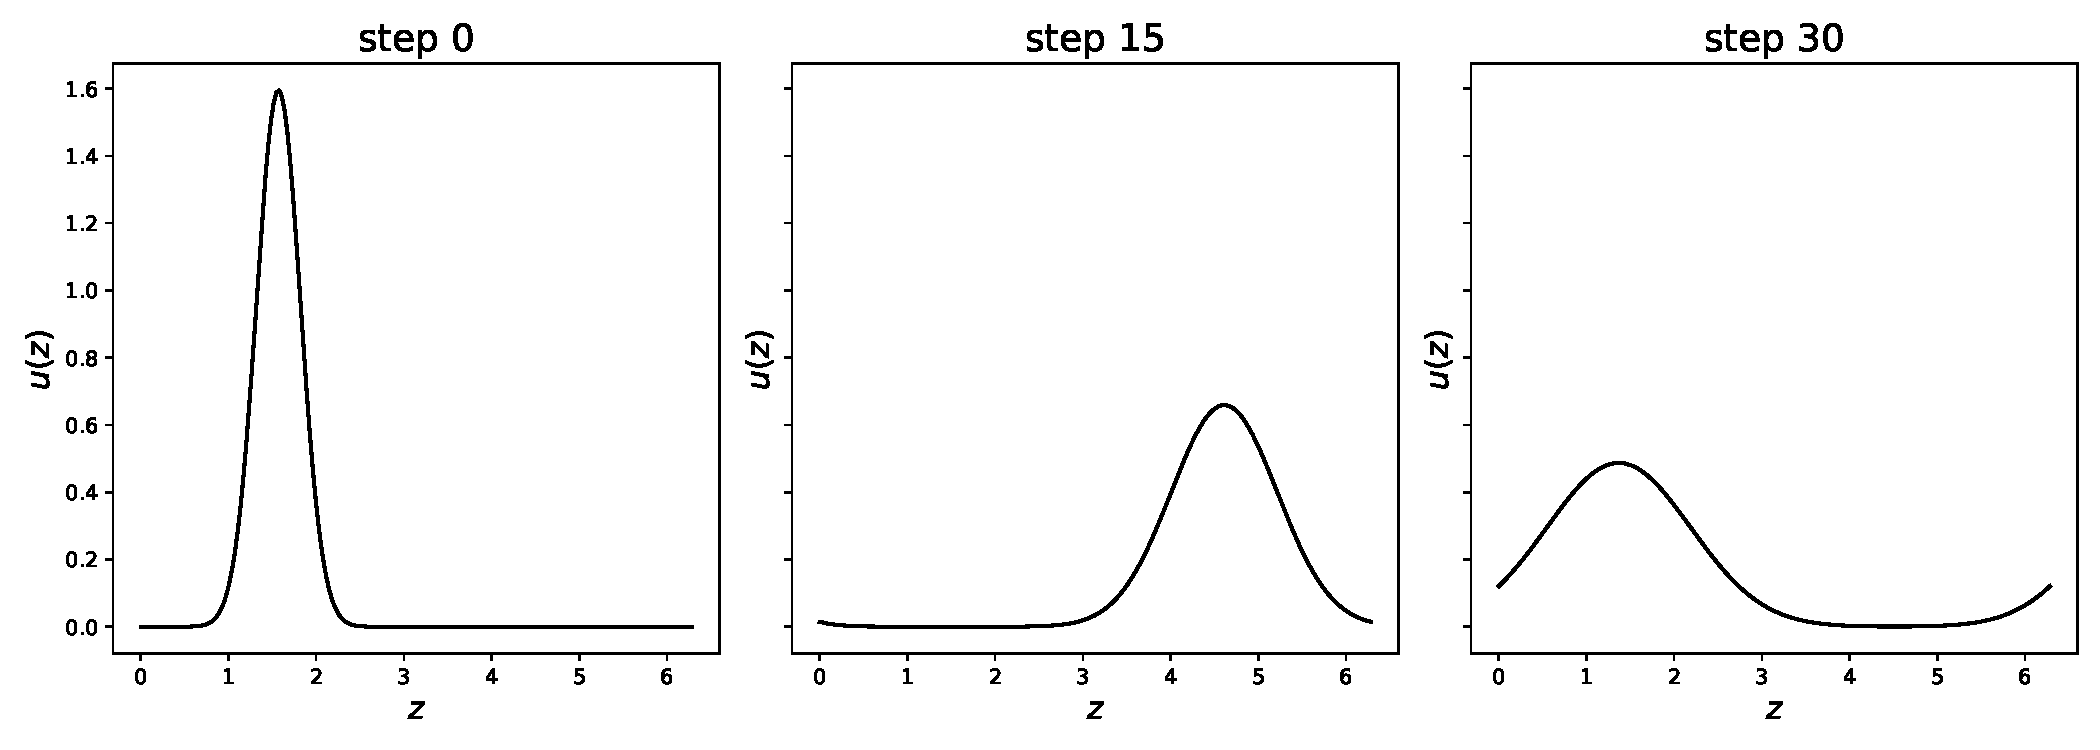
\includegraphics[width=\linewidth]{images/app1d/analytical_frame.pdf}
    \caption{La solution analytique du problème de convection-diffusion évolue au fil du temps.}
    \label{fig:1d_analytical}
\end{figure}

La forme lagrangienne des équations s'écrit

\begin{equation*}
    \frac{dx_p}{dt} = v(x_p, t), \quad \frac{dU_p}{dt} = D \frac{d^2 U_p}{dx^2}
\end{equation*}

Tout comme la méthode vortex décrite en Section~\ref{sec:vortex}, la résolution est réalisée en appliquant un schéma en deux étapes (\textit{viscous splitting}). où l'advection est réalisée au travers d'un schéma d'intégration euler explicite et l'opérateur laplacien est approché en toute position $\bx_p$ comme

\begin{equation*}
    \frac{dU_p}{dt} = D \varepsilon^{-d} V_p \sum_q (U_q - U_p) \phi_\varepsilon(x_q -  x_p),
\end{equation*}

% à mettre partie VIC
Le problème étant périodiques, nous définissons une fonction noyau équivalente $\phi_\varepsilon = \phi^P_g = \sum_{n=-\infty}^{+\infty} \phi_g(r - 2 \pi n)$.

Le modèle basé sur les particules utilise une discrétisation de \npart{} particules avec une taille de $h = \frac{L}{N_{\text{part}}}$ et une longueur de lissage de $\varepsilon = 1.3 h$.

Pour des raisons de comparaison, nous résolvons l'équation de convection-diffusion avec un schéma explicite de différences finies centrales discrétisé sur une grille régulière avec \ngrid{} nœuds.

\subsection{Paramètres d'assimilation et génération de l'ensemble}

\subsubsection{Distribution initiale}

On définit une distribution initiale pour le champ $u(\cdot, 0)$. A partir de cette distribution, un ensemble de taille  $N = 25$ membres est généré et resta commun aux différents fitres. Chaque membre par une fonction gaussienne définie par une moyenne et un écart-type différents. Egalement, les paramètres de l'équation d'évolution, la vitesse \(v\) et le coefficient de diffusion \(D\),  sont supposés inconnus. De cette manière une erreur de modèle est introduite et une calibration peut être réalisée. Les différentes distributions utilisées pour ces échantillons sont détaillées dans la Table~\ref{tab:ens_gen_1d}. Les paramètres échantillonnés et les états initiaux sont illustrés dans la Figure~\ref{fig:initial_gen}.

\begin{table}[htbp]
    \centering
    \caption{Ensemble generation variables}
    \begin{tabular}[t]{|l|l|}
        \hline
        Variables                   & Distributions                              \\
        \hline
        Gaussian mean               & $Z_m \sim  \mathcal{N}(\meanZm, \sigmaZm)$ \\
        Gaussian standard deviation & $S_m \sim\mathcal{U}(\smLow, \smUp)$       \\
        velocity                    & $v \sim \mathcal{N}(\vmean, \vstd)$        \\
        diffusion                   & $D \sim \mathcal{U}(\Dlow, \Dup)$          \\
        \hline
    \end{tabular}
    \label{tab:ens_gen_1d}
\end{table}

\begin{figure}[ht!]
    \centering
    \begin{subfigure}{0.49\textwidth}
        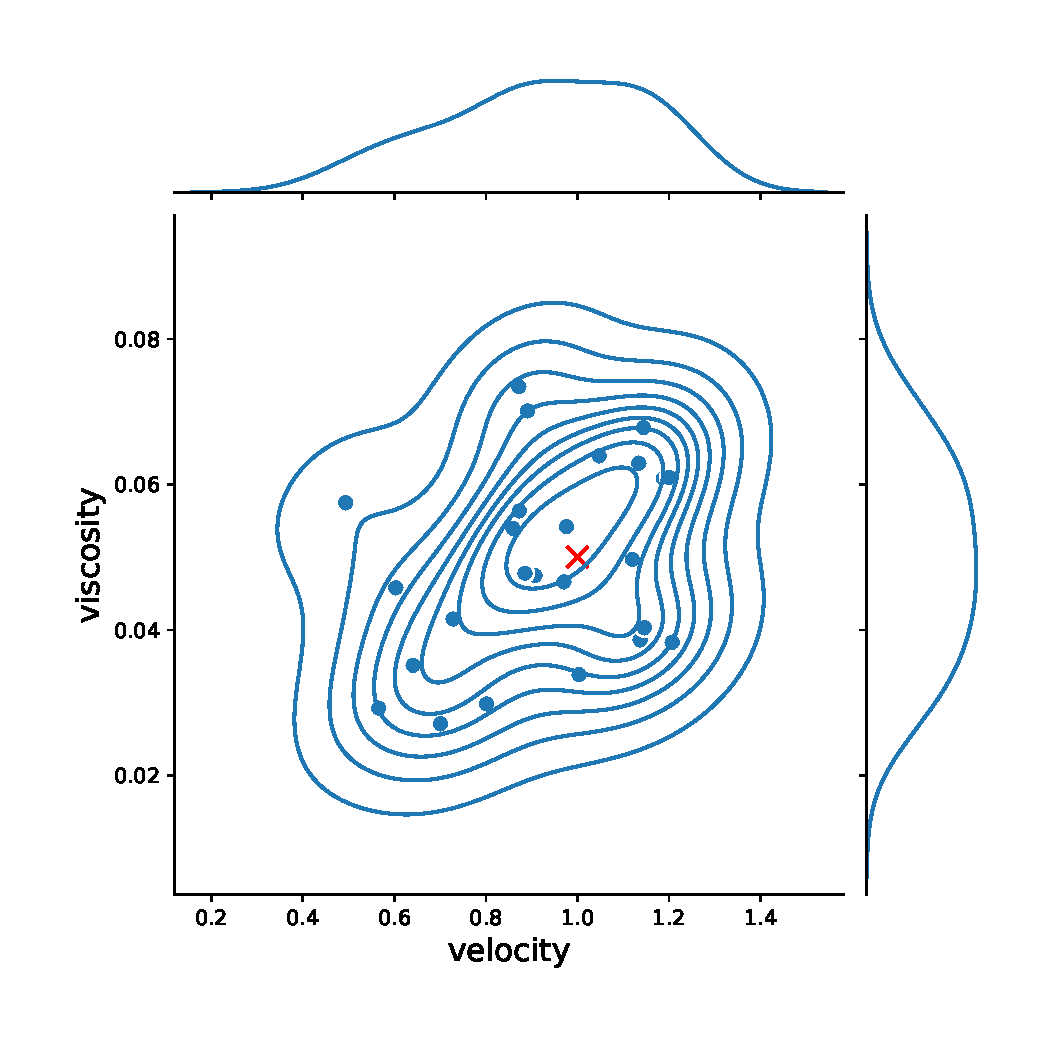
\includegraphics[width=\textwidth]{images/app1d/param.pdf}
    \end{subfigure}
    \hfill
    \begin{subfigure}{0.49\textwidth}
        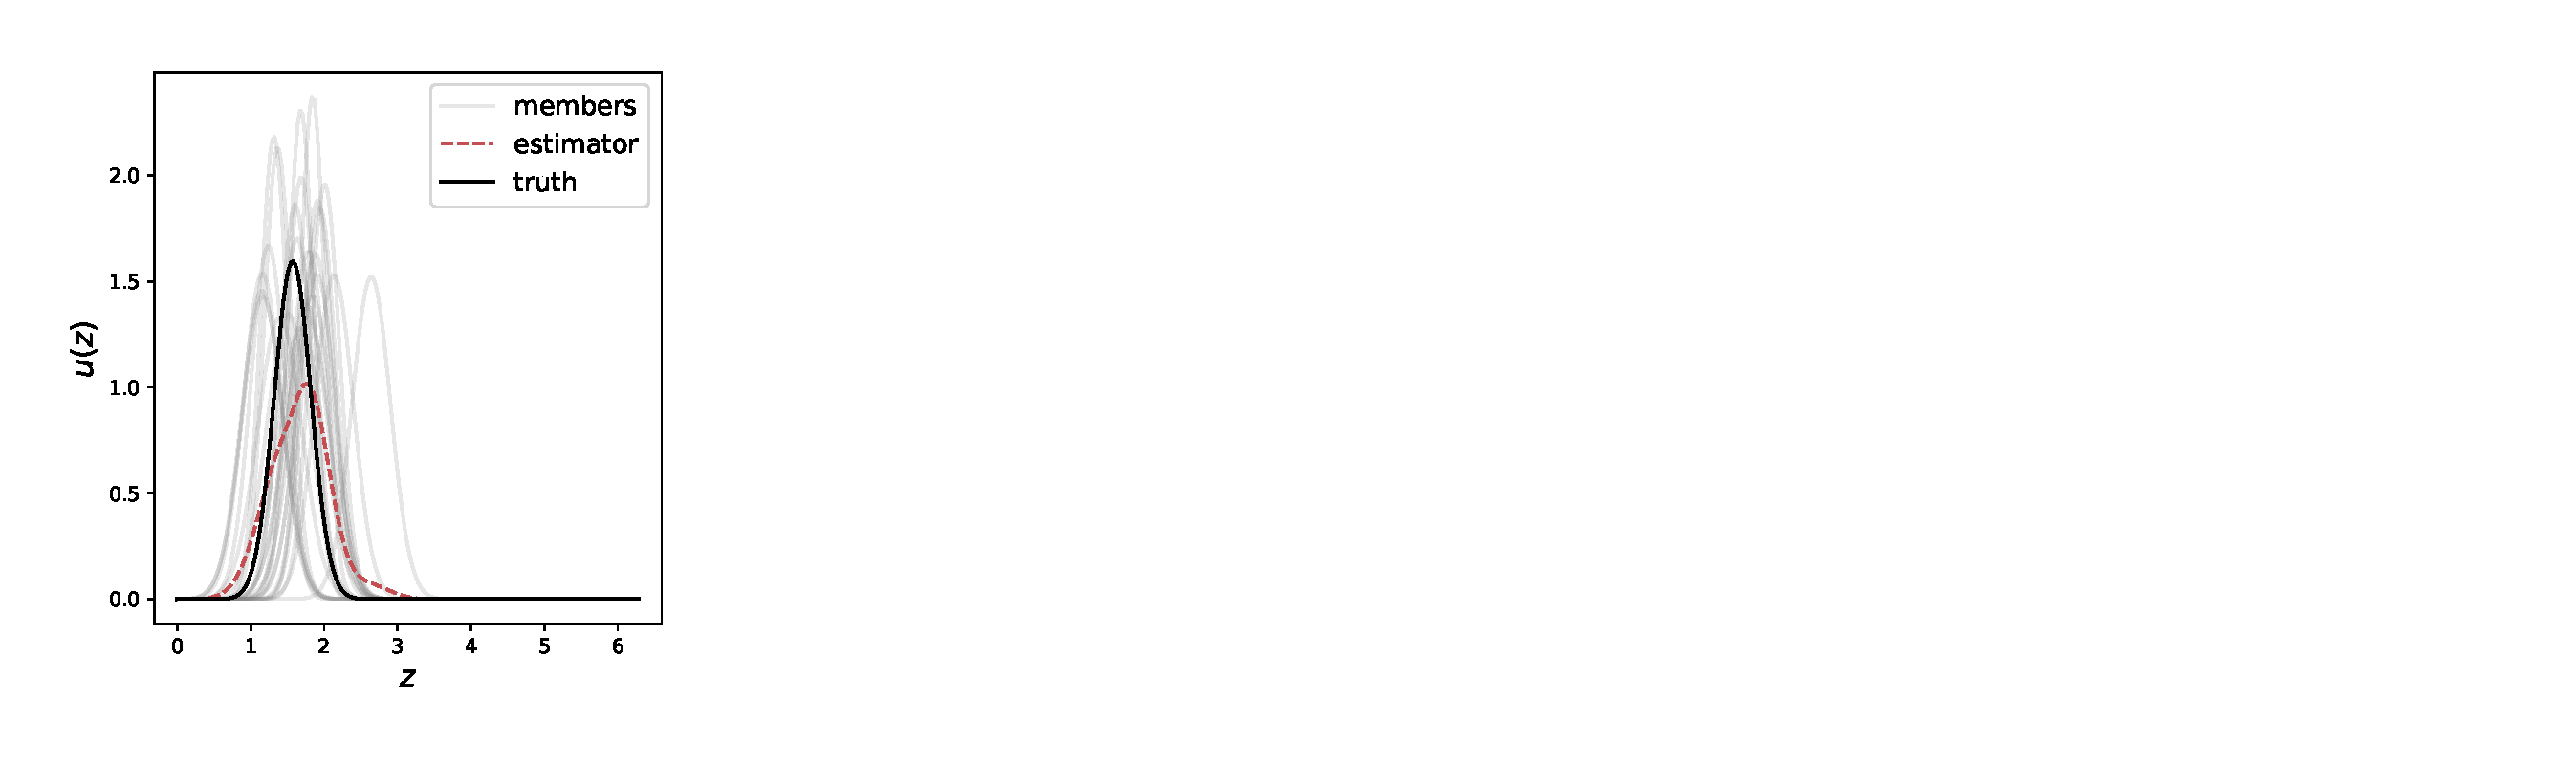
\includegraphics[width=\textwidth]{images/app1d/prior.pdf}
    \end{subfigure}
    \caption{On the left the initial parameters sample, $v$ in abscissa and $D$ in ordinate. On the right is the initial ensemble state.}
    \label{fig:initial_gen}
\end{figure}

Les données d'observation sont sujettes à un bruit additif, noté \(\eta \sim \mathcal{N}(0, \sigma_y \bm{I})\), où \(\sigma_y = \sigmaY\) et \(\bm{I}\) représente la matrice identité.

\subsubsection{Définition de l'erreur}

Nous définissons l'erreur comme le rapport relatif suivant

\begin{equation}~\label{eq:L2_error}
    e_{L_2} = \frac{\left[\frac{1}{\nens} \sum_{i = 1}^{\nens} \int_\Omega \left(u_i(z) - u^{gt}(z)\right)^2 dz\right]^{1/2}}{\norm{u^{gt}}_{L_2}}
\end{equation}
où \(u_i\) désigne le \(i\)-ème membre de l'ensemble et \(\norm{u}_{L_2}\) désigne la norme \(L_2\) de \(u^{gt}\).

La norme \(L_2\) est calculée en utilisant une quadrature sur une grille régulière d'un ensemble de cellules \(\mathcal{C}\) tel que pour tout \(f \in L_2\),

$$
    \norm{f}_{L_2} = \int_{\Omega} f^2~d\Omega \approx \sum_{c \in \mathcal{C}} f(z)~V_c
$$
où \(z_c\) est le centre de la cellule \(c\) et \(V_c\) le volume de la cellule. La grille reste la même pour toutes les simulations.

\subsubsection{Paramètres numériques}

Nous réalisons \(N_{\text{assim}} = 30\) étapes d'assimilation à intervalles réguliers jusqu'au temps final \(t_f = 2 \frac{L}{v}\). À chaque étape d'assimilation, le champ \(u^{gt}\) est observé à six positions régulièrement espacées \(x_{\text{obs}}\).

Dans la simulation basée sur des particules, les champs sont discrétisés en utilisant des particules régulièrement espacées mais avec un léger décalage. Les valeurs d'intensité sont obtenues en assignant la valeur d'intensité de particule $U_p = u(x_p) V_p$ de la même manière qu'en Section~\ref{sec:approx_part}. Cependant, le support particulaire de chaque membre sera différent. En effet, nous souhaitons évaluer notre méthode dans des situations où la discrétisation particulaire ne recouvre pas $\Omega$ dans sa totalité. Le support des particules semble déterminant pour le filtre Part-EnKF décrit en Section \ref{sec:part_enkf}. Ainsi, le paramètre \(\varepsilon_{\text{mass}}\) est introduit comme un seuil pour la sélection des particules, permettant de définir des nombres variables de particules pour chaque simulation.

Simultanément, une mise à jour standard de l'Ensemble Kalman Filter (EnKF) est appliquée aux variables nodales sur la simulation sur grille. Nous appellerons le filtre Grid-EnKF, le filtre EnKF utilisé pour la discrétisation sur grille. Pour la simulation basée sur une grille, les champs de chaque membre sont interpolés aux emplacements des nœuds. De cette manière, l'ensemble généré reste le même pour des fins de comparaison.

\subsection{Résultats}

Nous comparons les différents filtres sur l'assimilation de l'état. Nous comparons les différentes implémentation du filtre EnKF: le Grid-EnKF, le Remesh-EnKF, et deux filtres Part-EnKF avec un nombre de particules différents (100 et 60 particules). L'échantillon des paramètres reste inchangé. Nous prenons en compte les paramètres inconnus comme des incertitudes du modèle.

Dans la figure \ref{fig:1d_error_time}, nous apprécions les différentes étapes d'assimilation.

\begin{figure}
    \centering
    \begin{subfigure}{\textwidth}
        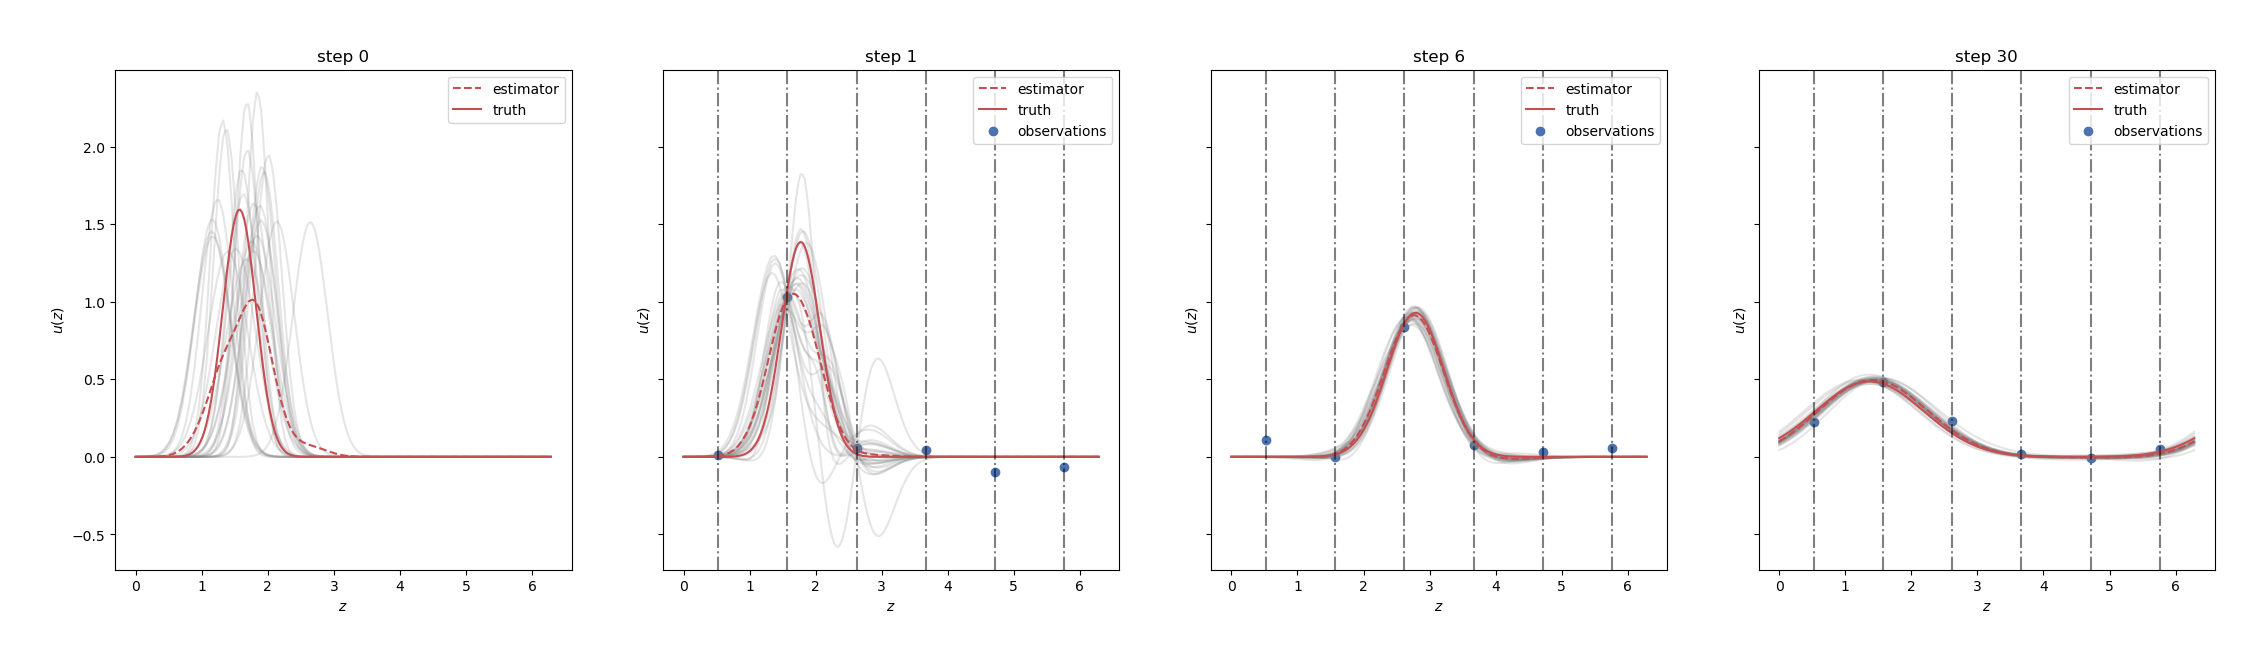
\includegraphics[width=\textwidth]{images/app1d/wo_calibration/grid_euler.png}
    \end{subfigure}
    \begin{subfigure}{\textwidth}
        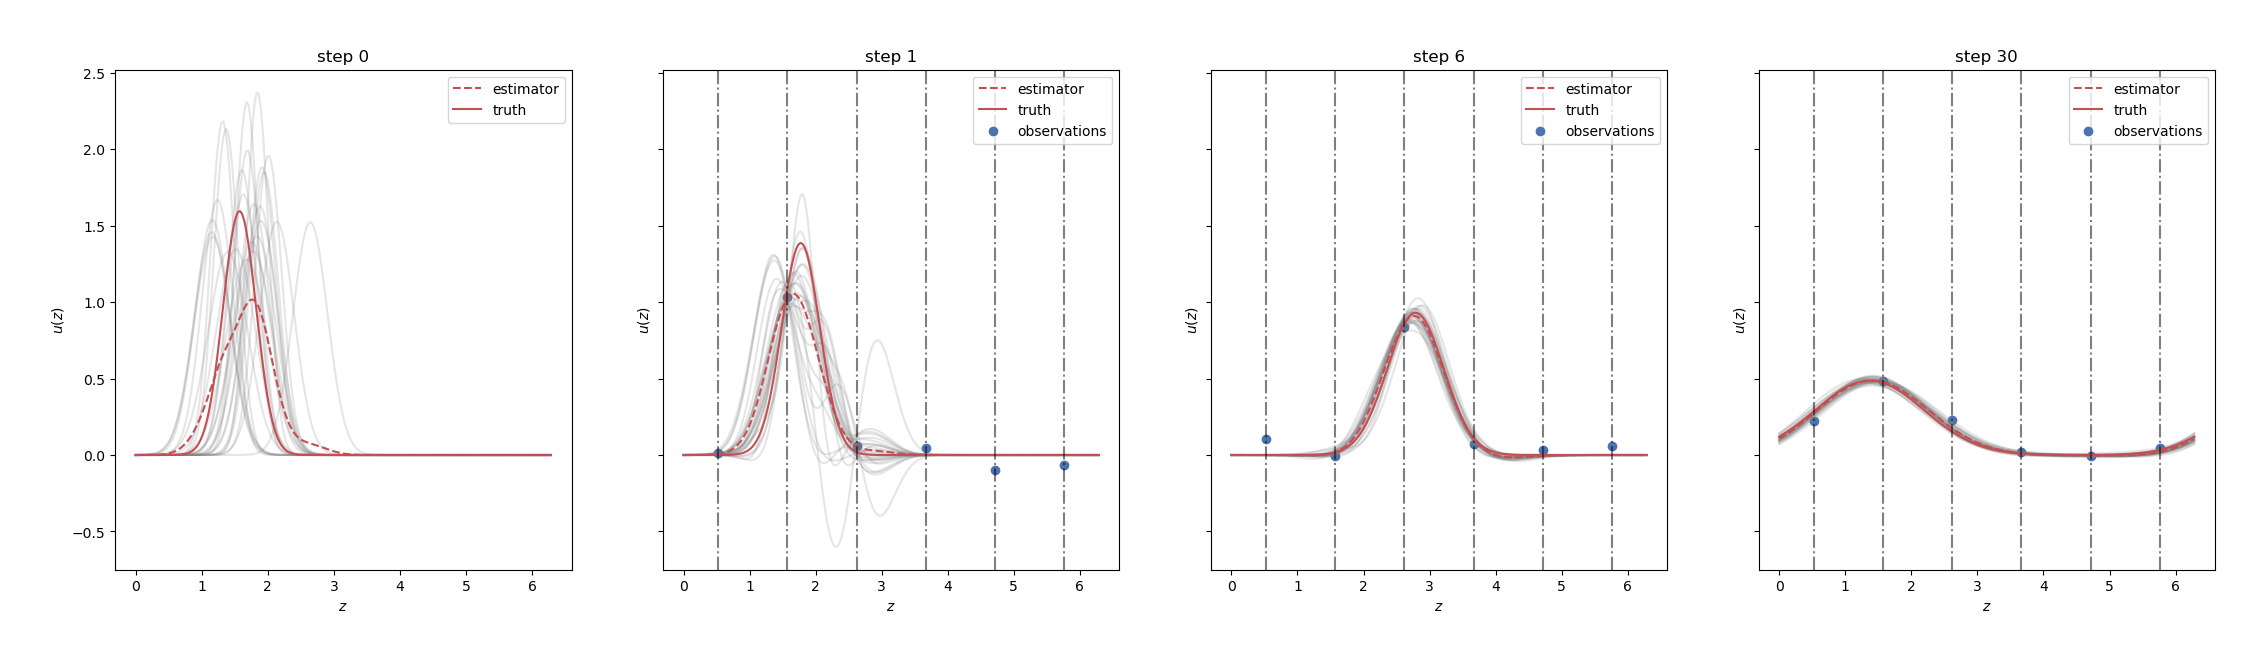
\includegraphics[width=\textwidth]{images/app1d/wo_calibration/remesh_EnKF.png}
    \end{subfigure}
    \begin{subfigure}{\textwidth}
        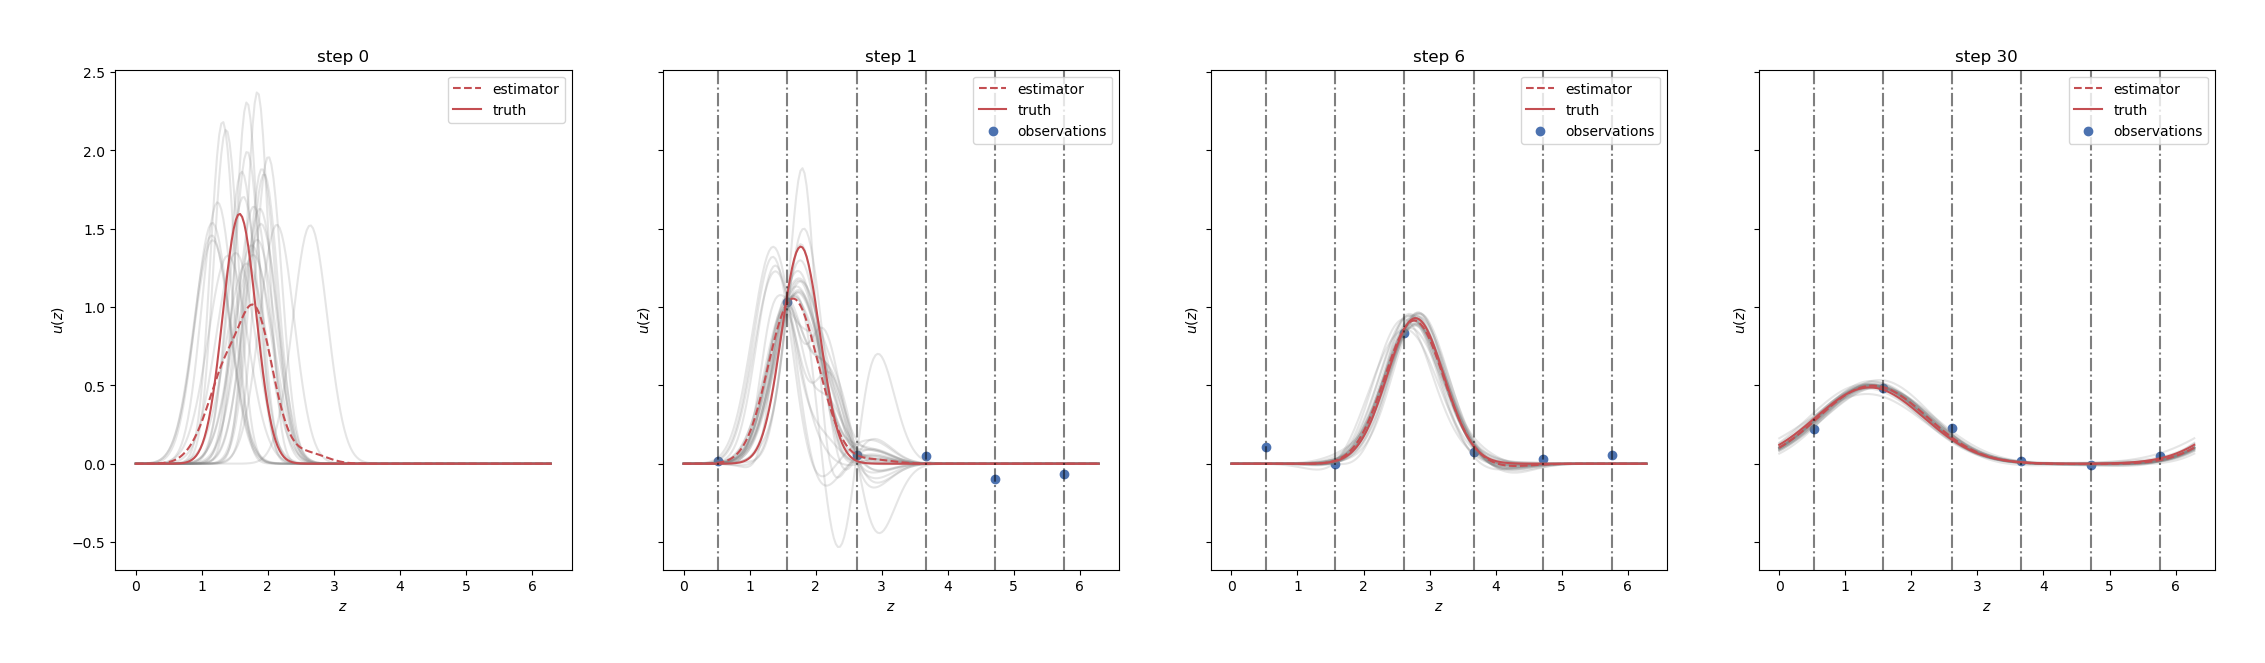
\includegraphics[width=\textwidth]{images/app1d/wo_calibration/part_enkf_30.png}
    \end{subfigure}
    \begin{subfigure}{\textwidth}
        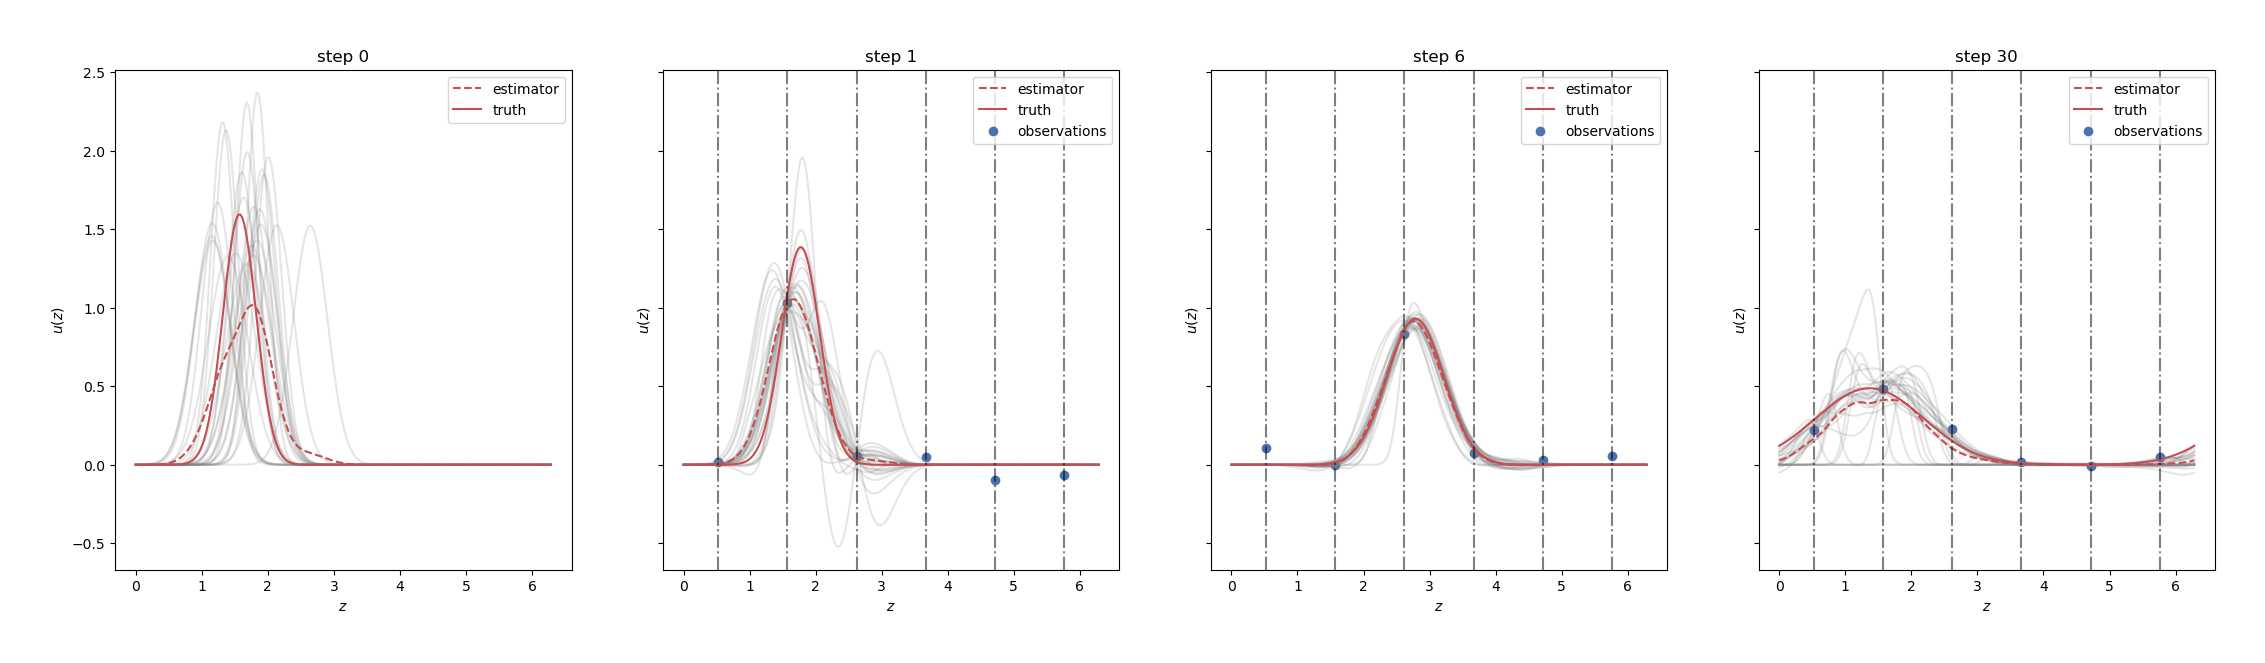
\includegraphics[width=\textwidth]{images/app1d/wo_calibration/part_enkf_60.png}
    \end{subfigure}
    \caption{Comparaison de l'assimilation des données entre différents filtres. De haut en bas : avec le filtre Grid-EnKF, le Remesh-EnKF, le Part-EnKF avec \(N_{\text{part}}=100\), et le Part-EnKF avec \(N_{\text{part}}=60\).}
\end{figure}
Le résultat est assez similaire pour tous les différents filtres. Néanmoins dans le cas où le support de particules est le plus faible, le filtre Part-EnKF avec 60 particules, le filtre ne converge pas. On retrouve quantitativement cette constatation sur la Figure~\ref{fig:1d_error_time}.

\begin{figure}
    \centering
    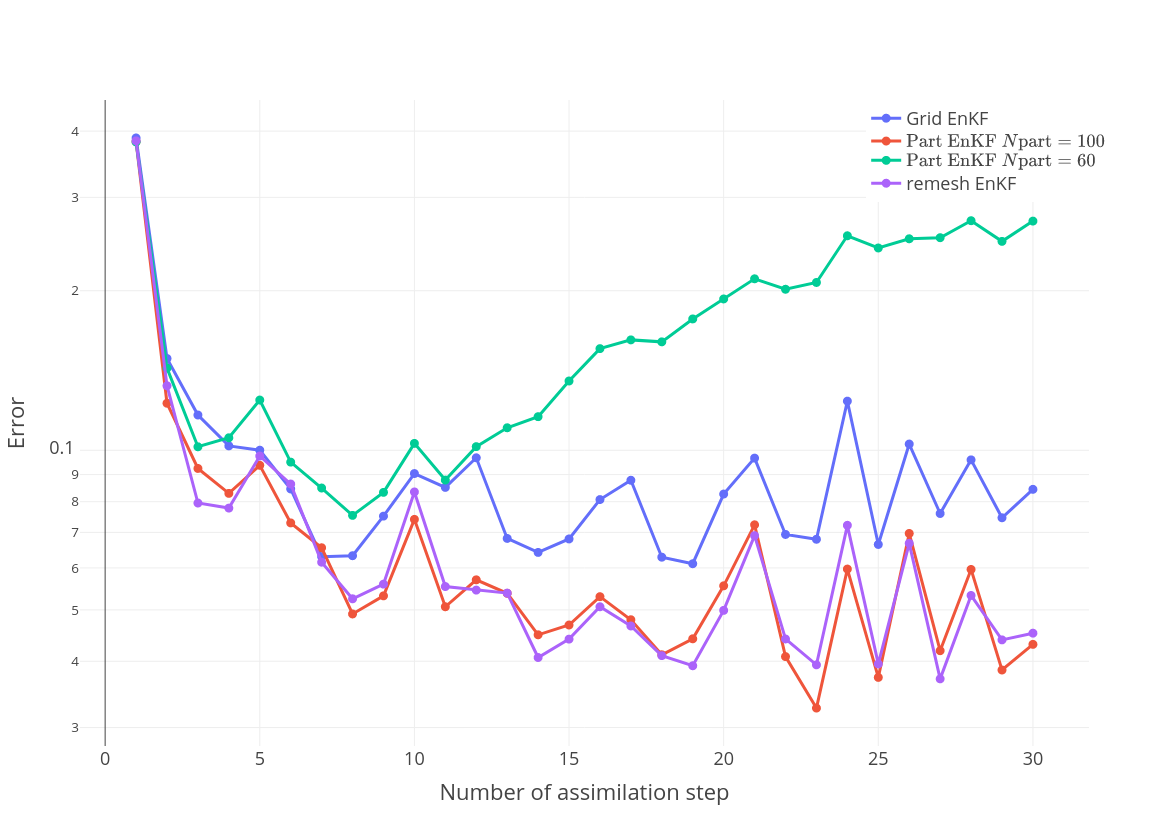
\includegraphics[width=0.75\textwidth]{images/app1d/wo_calibration/state_error.png}
    \caption{Erreur d'état en fonction du pas de temps d'assimilation.}
    \label{fig:1d_error_time}
\end{figure}

Le principal problème provient de la régression des champs analysés sur des supports de particules non conformes. Dans ce cas, la régression peine à ajuster les intensités de particule pour approcher le champ analysé définie sur un support de particules plus vaste. On observe en particulier une variabilité accrue au niveau la queue de la distribution.

Nous validons cette hypothèse en faisant varier le support initial des particules. Quantitativement, comme observé dans la Figure~\ref{fig:error_support}, l'estimation de l'erreur et la dispersion diminuent avec l'augmentation du nombre de particules. À partir de 70 particules, remarque
\begin{figure}
    \centering
    \begin{subfigure}{0.39\textwidth}
        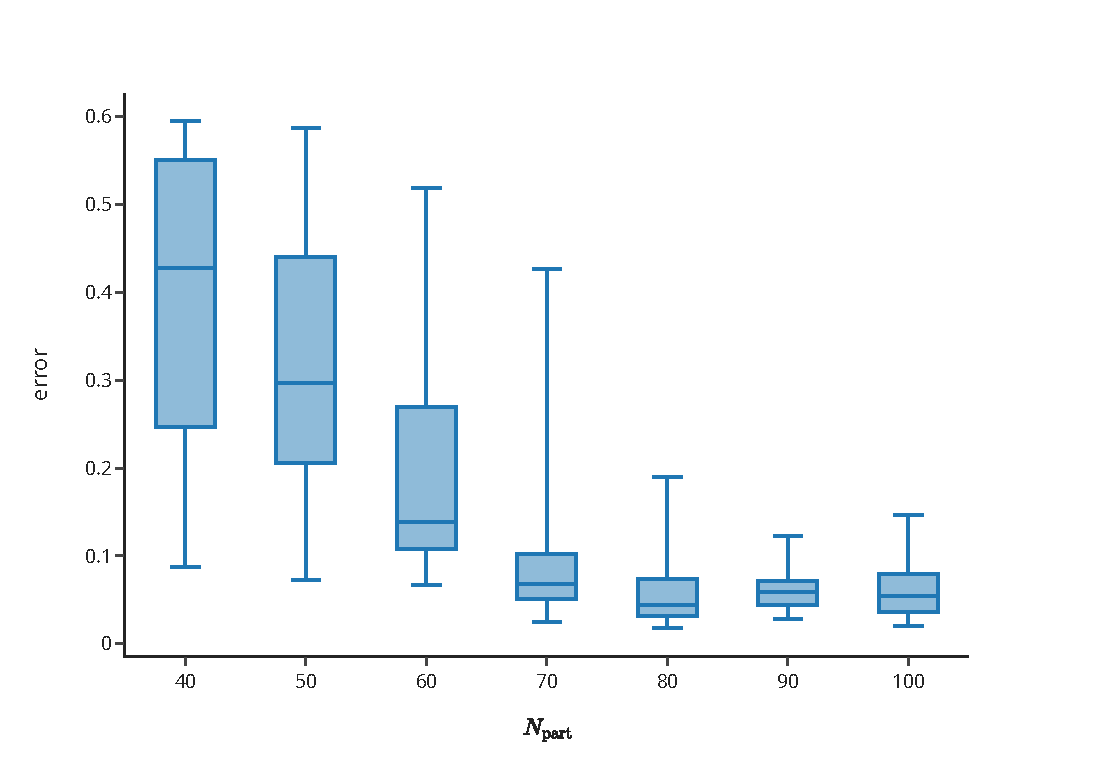
\includegraphics[width=\textwidth]{images/app1d/error_support/error_part.pdf}
        \caption{Erreur en fonction de la taille du support de particules.}
        \label{fig:error_support1}
    \end{subfigure}
    \hfill
    \begin{subfigure}{0.29\textwidth}
        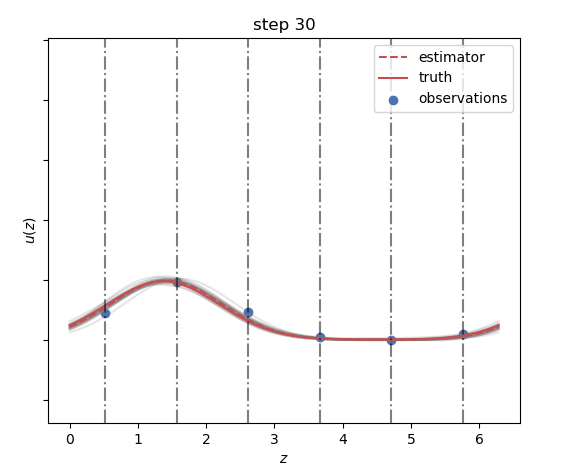
\includegraphics[width=\textwidth]{images/app1d/error_support/ok.png}
        \caption{Étape finale pour un support de 100 particules.}
        \label{fig:error_support2}
    \end{subfigure}
    \hfill
    \begin{subfigure}{0.29\textwidth}
        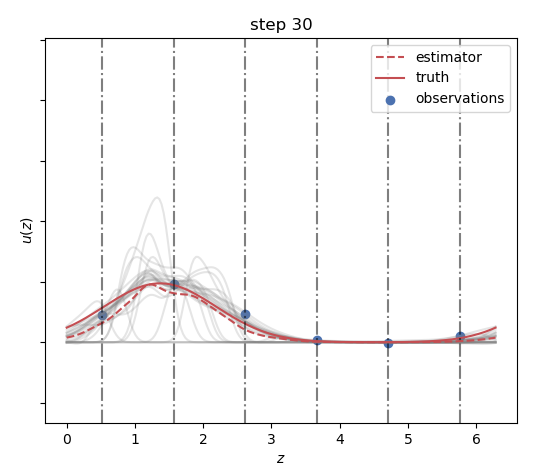
\includegraphics[width=\textwidth]{images/app1d/error_support/not_ok.png}
        \caption{Étape finale pour un support de 60 particules.}
        \label{fig:error_support3}
    \end{subfigure}
    \caption{À gauche : Erreur en fonction de la taille du support de particules. Au milieu : Étape finale pour un support de 100 particules. À droite : Étape finale pour un support de 60 particules.}
    \label{fig:error_support}
\end{figure}

Pour résoudre ce problème courant dans la régression par fonctions de base radiale (RBF)~\cite{fornberg_flyer_2015}, il est nécessaire d'augmenter le coefficient de pénalisation de la régression \textit{Ridge}.

Même avec une régression plus stable, elle reste une projection de la solution d'analyse sur le précédent jeu de particule, le seul moyen d'amélioration de la solution est donc d'ajouter des particules supplémentaires.

Cependant, l'ajout de particules reste quelque chose de complexe, pourfois même impossible. De plus, il est alors nécessaire de préserver un bon espacement entre les particules et une densité particulaire adéquate. De plus, le filtre Part-EnKF a été introduit justement pour traiter le cas où la génération de nouvelles particules ne serait pas possible.

Ainsi, si pour le filtre Part-EnKF, l'erreur de reconstruction est trop importante (par exemple en évaluant l'écart sur un nouveau jeu de particules) et si la génération de particule est possible, alors il préférable d'utiliser alors le filtre Remesh-EnKF

En conclusion, cet exemple souligne la capacité du filtre Remesh-EnKF à produire des résultats comparables à ceux de l'EnKF classique appliqué à un modèle de grille. De plus, il met en évidence la capacité du Part-EnKF à assimiler une discrétisation par particules tout en soulignant l'importance de prendre en compte la répartition spatiales des particules inter et intra membres.

\section{Problème 2D}

\subsection{Description du problème}

Dans cette section nous évaluons le résultat des deux types de filtre sur un problème bi-dimensionnel en utilisant la méthode vortex comme décrite en Section~\ref{sec:vortex}.

Nous procédons à l'assimilation du problème d'advection d'un dipôle de Lamb-Chaplygin au sein d'un domaine fermé $[0, \pi]^2$. Le dipôle de Lamb-Chaplygin est un choix populaire pour les études numériques~\cite{orlandi_vortex_1990}. Le modèle représente un écoulement dipolaire spécifique, stationnaire, offrant une solution non triviale aux équations d'Euler bidimensionnelles dans le cas non visqueux. Ce qui d'autant plus interessant est que ce dipôle est caractérisé par une vitesse de translation \(U\), une position moyenne \(\bm{z}_0\), un rayon \(R\) et une orientation \(\alpha\).

Le champ de vorticité du dipôle \(\omega\) peut être exprimé comme

\begin{equation*}
    \omega(r) = \begin{cases}
        \frac{-2 k U J_1(kr)}{\omega J_0(kR)} \sin \alpha \quad & \text{pour} \quad r < R, \\
        0 \quad                                                 & \text{sinon},
    \end{cases}
\end{equation*}
où \((r, \alpha)\) représentent les coordonnées polaires dans le référentiel du dipôle. Ici, \(J_0\) et \(J_1\) désignent respectivement les fonctions de Bessel de premier type d'ordre zéro et d'ordre un, et \(k\) est déterminé de sorte que \(kR\) corresponde au premier zéro non trivial de la première fonction de Bessel. Le champ de vorticité du dipôle est illustré dans la Figure \ref{fig:lamb_dipole}.

\begin{figure}[ht]
    \centering
    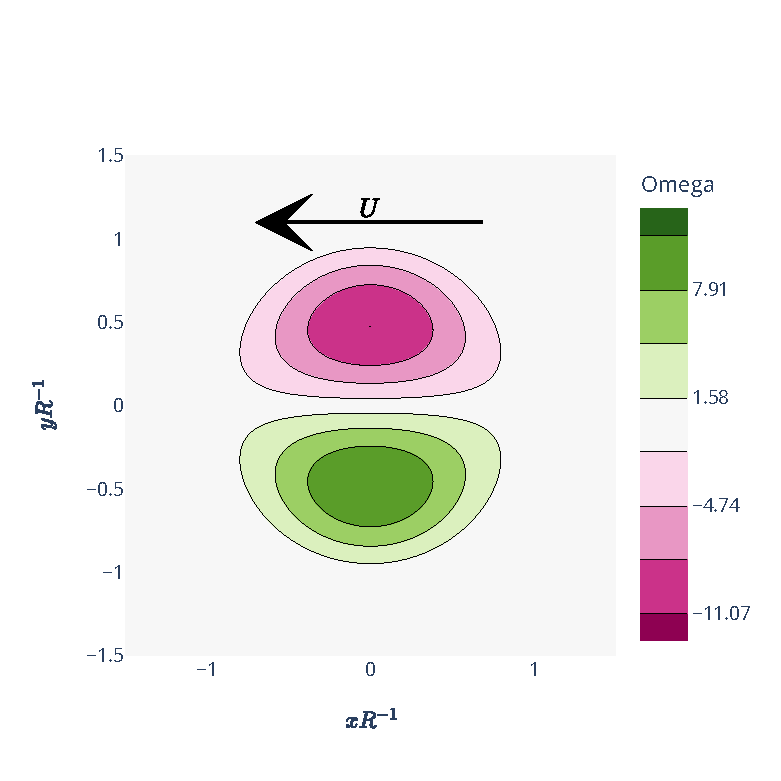
\includegraphics[width=0.6\linewidth]{images/app2d/lamb.pdf}
    \caption{The Lamb-Chaplygin dipole vorticity field on a normalized space.}
    \label{fig:lamb_dipole}
\end{figure}

Le dipole est initialement positionné au centre du domaine avec une orientation de \(\frac{7\pi}{8}\) rad, un rayon de 0.5m et une vitesse \(U\) de 0.25 \(\text{m.s}^{-1}\). Les paramètres de référence complets sont listés dans le Tableau \ref{tab:ref}.

\begin{table}[htbp]
    \centering
    \caption{Paramètres de référence}
    \begin{tabular}[t]{|l|l|}
        \hline
        Paramètres               & Valeurs                                                              \\
        \hline
        viscosité de référence   & $v_{\text{ref}} = 0.001$                                             \\
        orientation de référence & $\theta_{\text{ref}}  = \frac{7 \pi}{8} (\text{rad.})$               \\
        position du barycentre   & $\bm{z}_{\text{ref}} = \left[\frac{\pi}{2}, \frac{\pi}{2} \right]^T$ \\
        vitesse de translation   & $U_{\text{ref}} = 0.25$                                              \\
        \hline
    \end{tabular}
    \label{tab:ref}
\end{table}

Aux frontières, la vitesse normale aux parois est nulle, tandis que la vitesse tangentielle reste indéterminée.

Comme ce problème n'a pas de solution explicite dans un domaine fermé, nous simulons la vérité terrain avec la méthode des vortex pour une discrétisation fine et un ensemble de paramètres fixes également décrits dans le Tableau \ref{tab:ref}. La trajectoire de la vérité terrain est illustrée dans la Figure \ref{fig:ref_trajectory} sur une grille régulièrement espacée.

\begin{table}[htbp]
    \centering
    \caption{Paramètres nominaux d'assimilation et de simulation}
    \begin{tabular}[t]{|l|l|}
        \hline
        Paramètres                              & Valeurs                                     \\
        \hline
        pas de temps                            & $dt = 0.005$                                \\
        temps final                             & $t_f = 10$                                  \\
        écart-type de l'observation             & $\sigma_{obs} =  5.0 \times 10^{-2}$        \\
        seuil de vorticité                      & $\varepsilon_{\omega} = 1.0 \times 10^{-4}$ \\
        longueur caractéristique des particules & $dp = \frac{\pi}{256} \approx 0.01227 $     \\
        longueur de lissage                     & $h = 2.0 \, dp$                             \\
        nombre d'assimilations                  & $N_{\text{assim}} = 10$                     \\
        taille de l'ensemble                    & $N_{\text{ens}} = 32$                       \\
        nombre d'observations                   & $N_{\text{obs}} = 12^2 = 144$               \\
        discrétisation de la grille             & $N_{\text{grid}} = 65^2 = 4225$             \\
        % nombre de remaillages par prévision     & $N_{\text{remesh}} = 2 $                    \\
        \hline
    \end{tabular}
    \label{tab:simu_2d}
\end{table}

\begin{figure}[htbp]
    \begin{subfigure}{0.32\textwidth}
        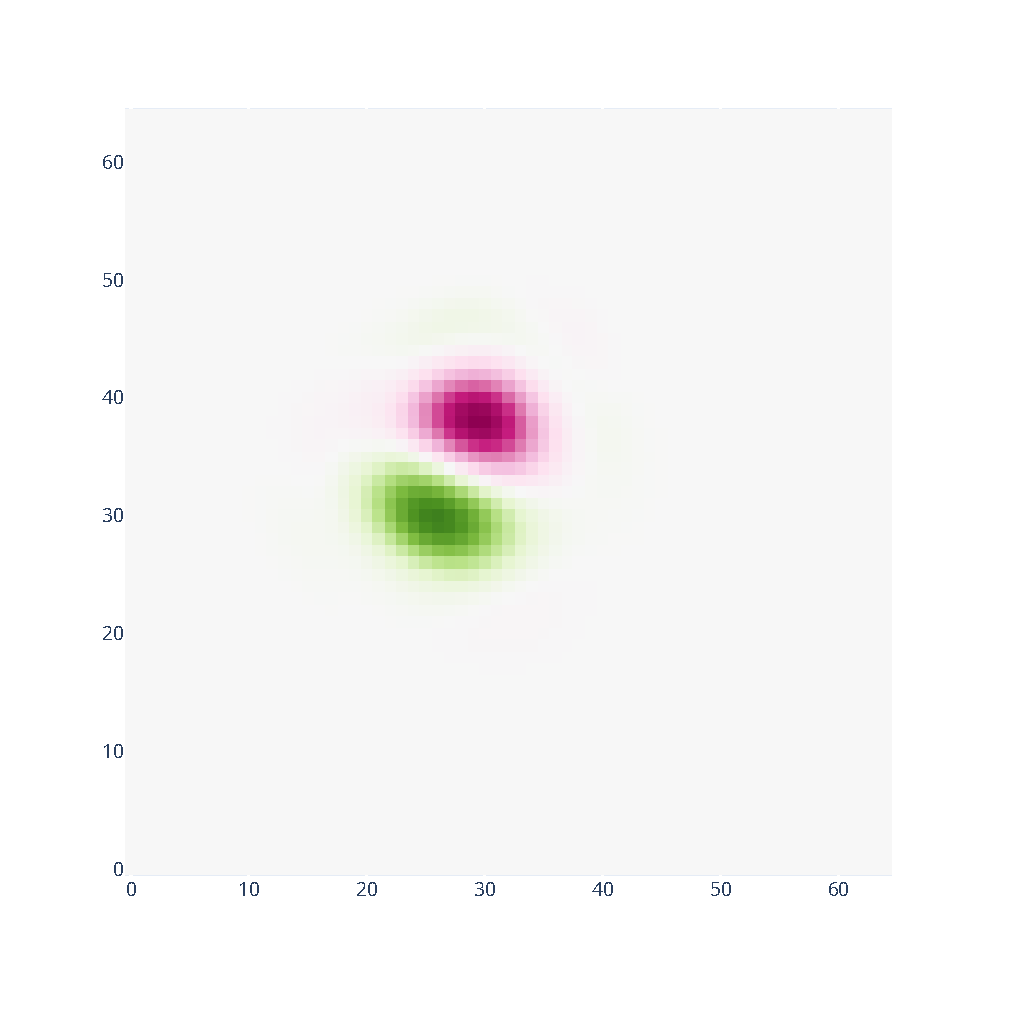
\includegraphics[width=\linewidth]{images/app2d/best_estimate_2.pdf}
    \end{subfigure}
    \hfill
    \begin{subfigure}{0.32\textwidth}
        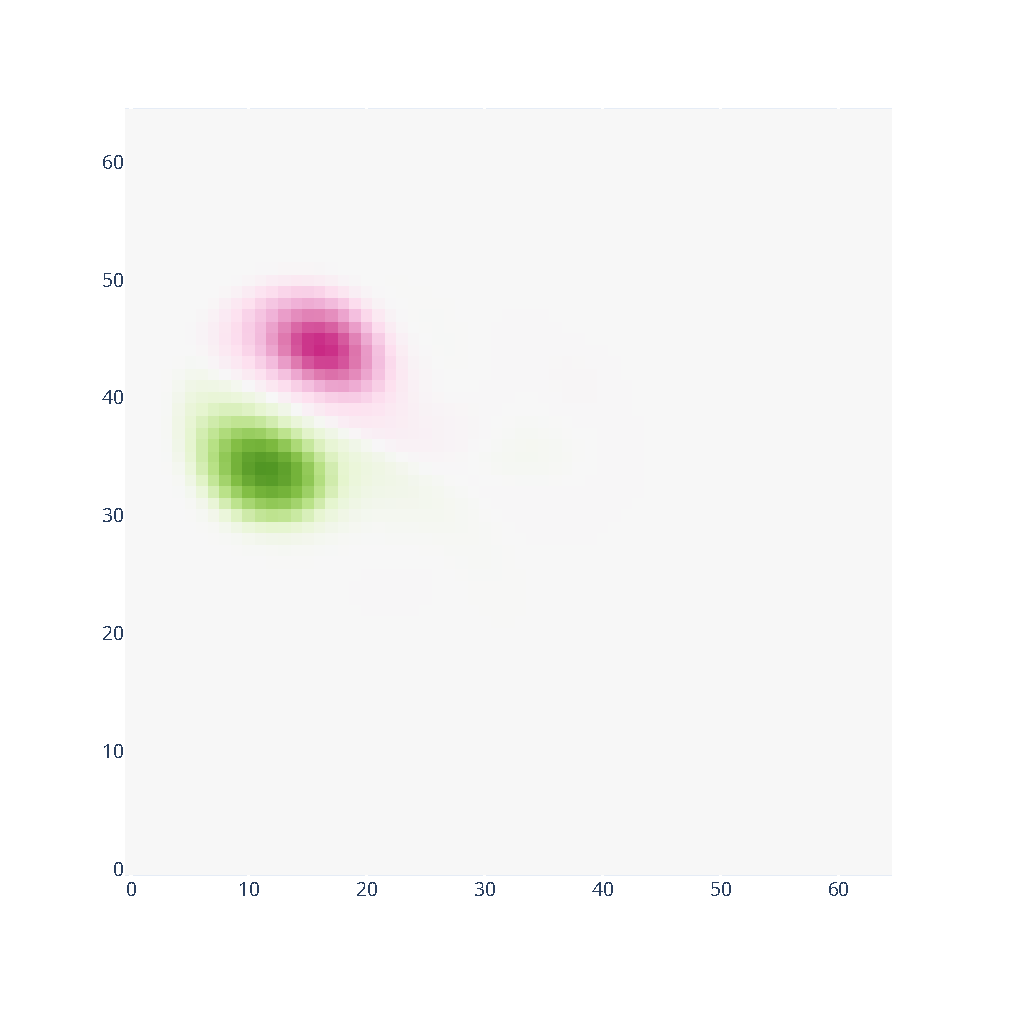
\includegraphics[width=\linewidth]{images/app2d/best_estimate_10.pdf}
    \end{subfigure}
    \hfill
    \begin{subfigure}{0.32\textwidth}
        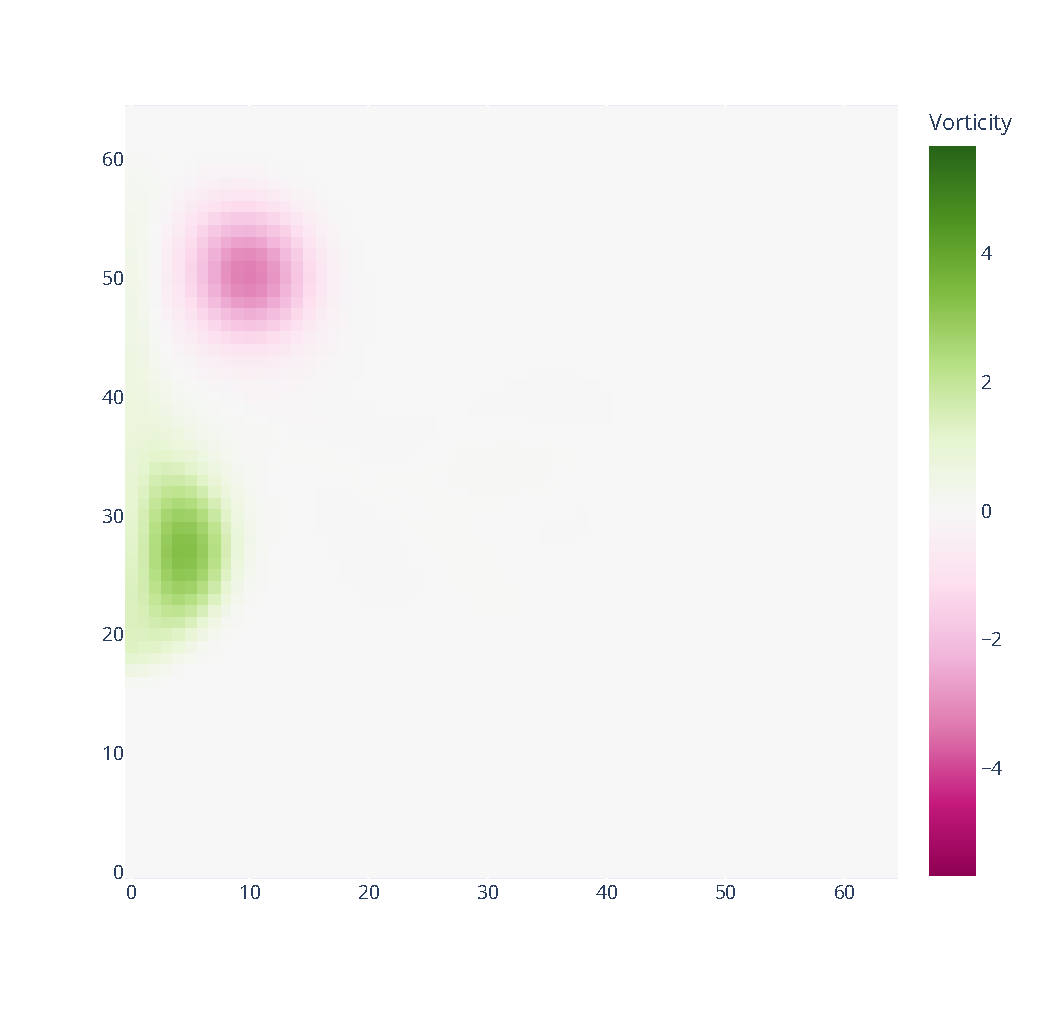
\includegraphics[width=\linewidth]{images/app2d/best_estimate_20.pdf}
    \end{subfigure}
    \caption{Trajectoire de la vérité terrain. La vorticité est représentée sur une grille régulièrement espacée. Pour $t=[1, 5, 10]$ s.}
    \label{fig:ref_trajectory}
\end{figure}


Plusieurs paramètres de la simulation influencent la distribution des particules et peuvent conduire à des résultats différents. Le premier est la taille des particules définie par \(d_p\). Un autre paramètre significatif est \(\varepsilon_\omega\), associé au processus de remaillage se produisant soit pendant la prévision (pour éviter une distorsion élevée de la distribution des particules) soit pendant le filtre Remesh-EnKF. \(\varepsilon_\omega\) sert de seuil, déterminant si une particule est retenue après le processus de remaillage basé sur la condition \(V_p \Gamma_p > \varepsilon_\omega\). L'impact de ce paramètre est illustré pour un membre après la première prévision dans la Figure~\ref{fig:eps_effect}.

\begin{figure}[htbp]
    \centering
    \begin{subfigure}{0.3\textwidth}
        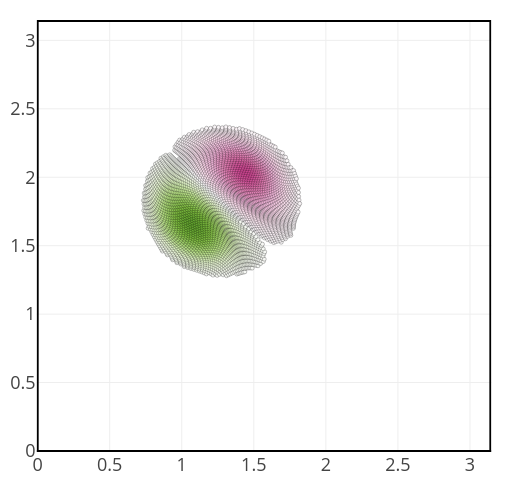
\includegraphics[width=\linewidth]{images/app2d/part_eps_0.1.png}
    \end{subfigure}
    \hfill
    \begin{subfigure}{0.3\textwidth}
        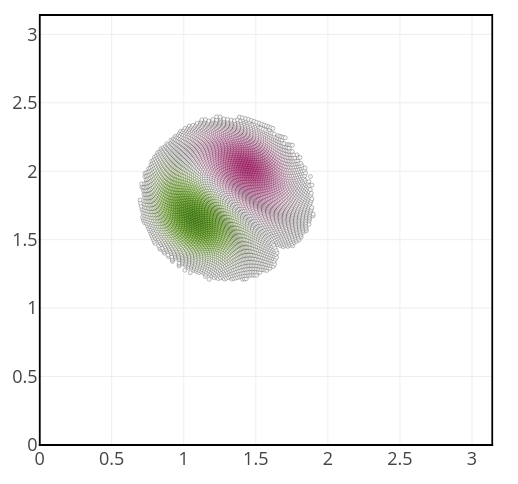
\includegraphics[width=\linewidth]{images/app2d/part_eps_0.01.png}
    \end{subfigure}
    \hfill
    \begin{subfigure}{0.3\textwidth}
        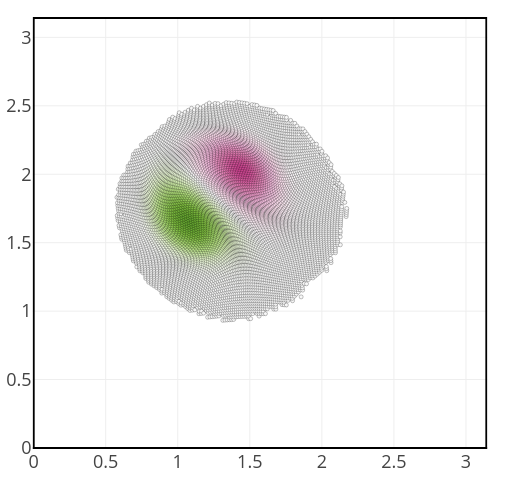
\includegraphics[width=\linewidth]{images/app2d/part_eps_1e-6.png}
    \end{subfigure}
    \caption{Effet du paramètre $\varepsilon_\omega$ sur la discrétisation des particules de la solution pour un membre. De gauche à droite, résultats pour $\varepsilon_\omega = 0.1, 0.01$ et $1.e^{-6}$.}
    \label{fig:eps_effect}
\end{figure}


\subsection{Paramètres d'assimilation et génération d'ensemble}

\subsubsection{Distribution d'ensemble}
Nous générons un ensemble initial de 32 membres en échantillonant une distribution de paramètre du dipole.

Nous échantillonnons le rayon \(R\), la vitesse prescrite \(U\), l'orientation \(\alpha\) et le barycentre \(\bm{z}_{\text{mean}}\). De plus, la viscosité du modèle \(\nu\) est également échantillonnée. Toutes les distributions sont résumées dans le Tableau \ref{tab:ens_dipole}. Les six premiers membres sont représentés dans la Figure \ref{fig:sample_ens}.

\begin{table}[htbp]
    \centering
    \caption{Variables de génération de l'ensemble}
    \begin{tabular}[t]{|l|l|}
        \hline
        Variables   & Distributions                                                                                                                                  \\
        \hline
        rayon       & $R \sim \mathcal{N}(1.0, 0.05^2)$                                                                                                              \\
        orientation & $\theta \sim \mathcal{U}\left(\pi, \frac{\pi}{2} \right) (\text{rad.})$                                                                        \\
        barycentre  & $z_{\text{mean},x} \sim \mathcal{N}\left(\frac{\pi}{2},0.1^2\right), \quad z_{\text{mean},y} \sim \mathcal{N}\left(\frac{\pi}{2},0.1^2\right)$ \\
        vitesse     & $U \sim \mathcal{U}(0, 0.5^2)$                                                                                                                 \\
        viscosité   & $v \sim \mathcal{N}(0.0015, 0.0005^2)$                                                                                                         \\
        \hline
    \end{tabular}
    \label{tab:ens_dipole}
\end{table}

\begin{figure}[ht]
    \centering
    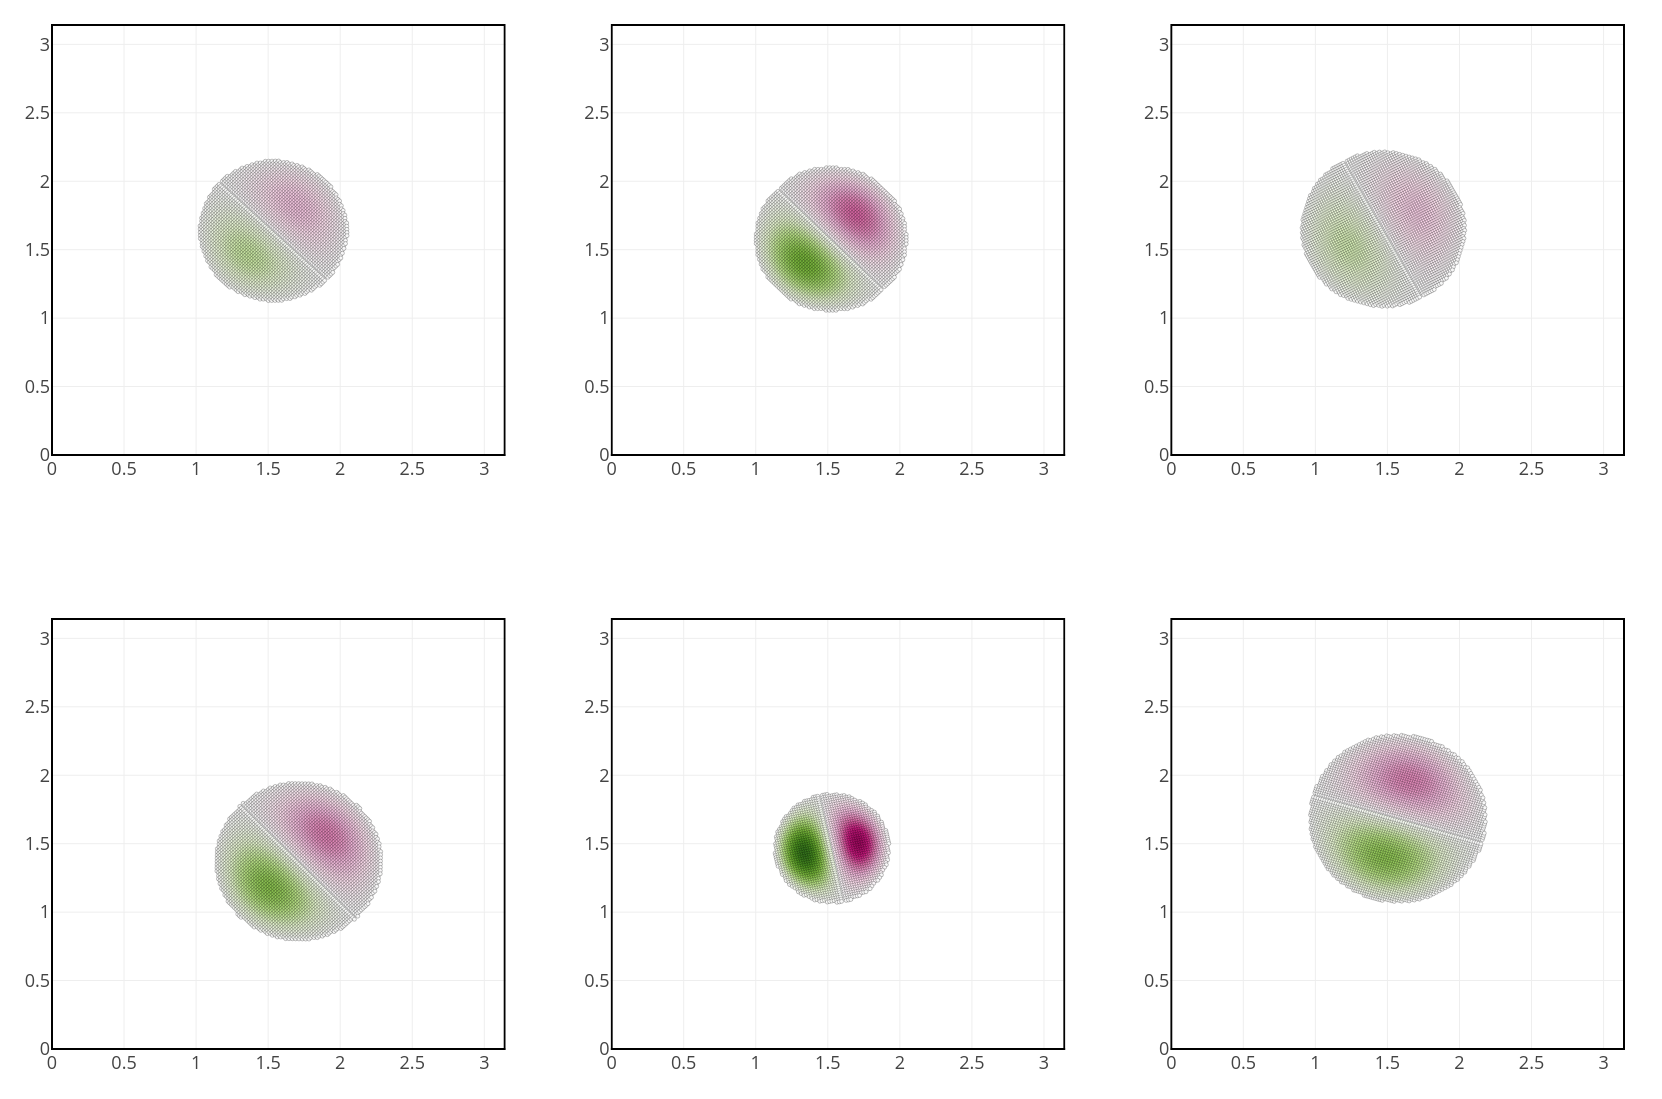
\includegraphics[width=0.9\linewidth]{images/app2d/ensemble_sample.png}
    \caption{Six échantillons de l'ensemble initial.}
    \label{fig:sample_ens}
\end{figure}

Le champ de vorticité initial est d'abord discrétisé sur une grille régulière de particules avec une longueur caractéristique \(d_p\), où chaque particule reçoit la circulation \(\Gamma_p = \omega(\bm{z}_p) V_p\) et \(V_p = d_p^2\) représente le volume de la particule.

\subsubsection{Définition de l'erreur}

Nous utilisons une erreur absolue \(L_2\) définie par $ \frac{1}{\nens} \sum_{i = 1}^{\nens} \int_\Omega \left(\omega_i(\bm{z}) - \omega^{gt}(\bm{z})\right)^2 \mathrm{d}\bm{z}$. Nous utilisons également les erreurs des membres pour évaluer la dispersion de l'estimation de l'erreur.

\subsubsection{Paramètres numériques}

La fréquence d'assimilation est définie par le pas d'assimilation $dt_a$. La simulation est effectuée sur une durée de $t_f$. Tous les paramètres de simulation sont résumés dans le Tableau \ref{tab:simu_2d}.

Les observations sont collectées sur une grille régulière de taille $N_{\text{obs}}$, mesurant les deux composantes de la vitesse. Les observations suivent une distribution normale $\mathcal{N}(0, \sigma_{\text{obs}}^2 \bm{I})$, indiquant un ensemble de mesures indépendantes, chacune caractérisée par une distribution standard de $\sigma_{\text{obs}}$. Un exemple de vitesse observée avec et sans bruit est illustré dans la Figure \ref{fig:velocity}.

\begin{figure}[htbp]
    \centering
    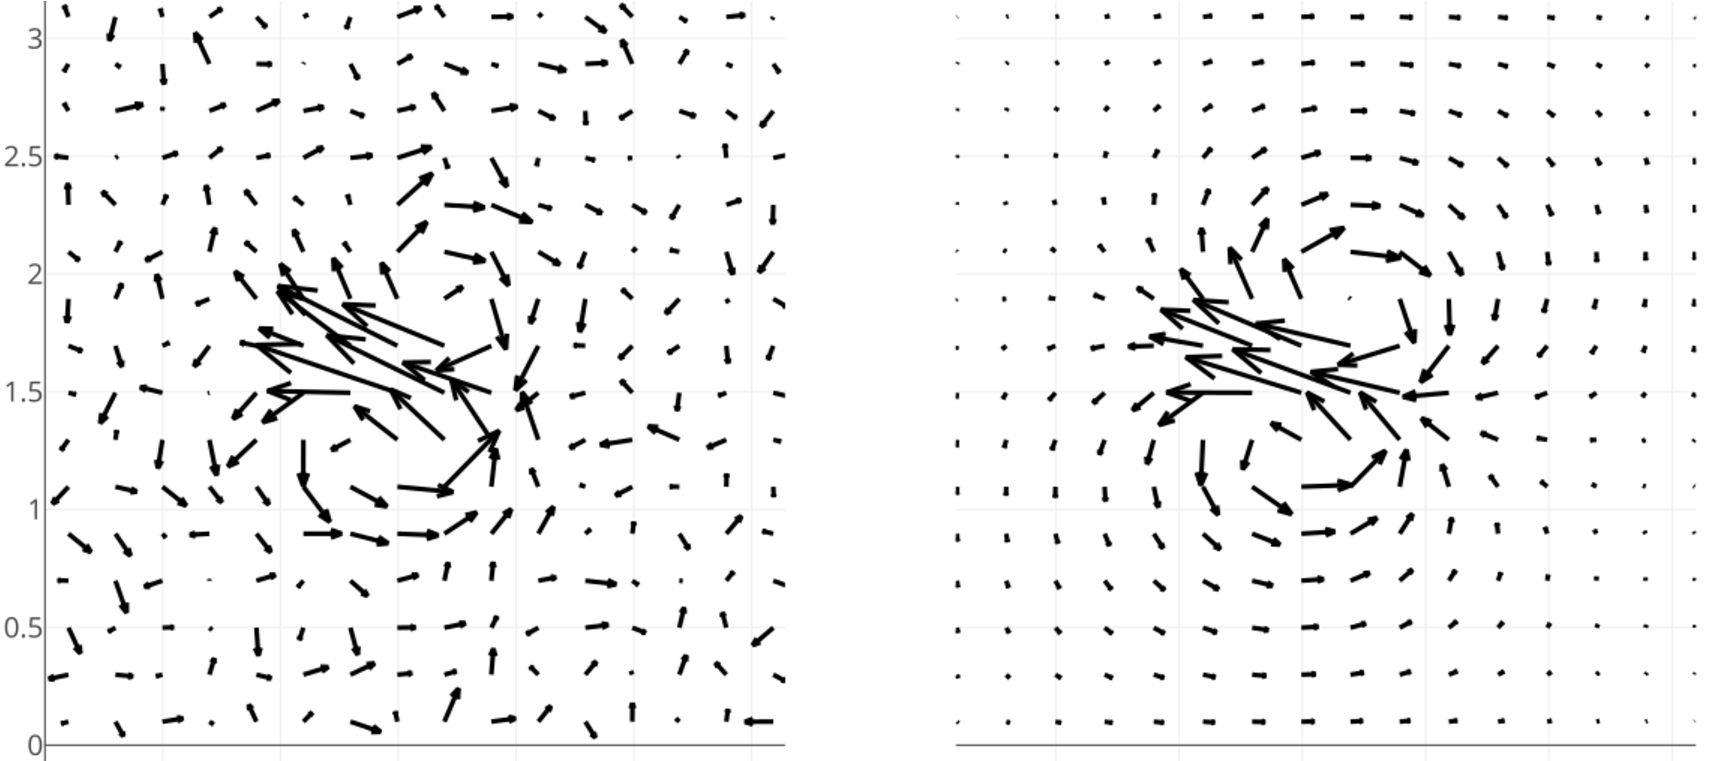
\includegraphics[width=0.8\linewidth]{images/app2d/velocity_ref_recadre.pdf}
    \caption{Champs de vitesse observés et de référence. L'erreur sur chaque composante est un échantillon d'une distribution normale centrée avec la valeur nominale $\sigma_{\text{obs}} = 0.05$.}
    \label{fig:velocity}
\end{figure}

\subsection{Résultats}

\subsection{Assimilation au cours du temps}

Nous commençons par analyser l'erreur d'assimilation au cours du temps. La Figure~\ref{fig:assim_time} illustre l'erreur tout au long du processus d'assimilation pour l'ensemble nominal de paramètres d'assimilation, montrant des résultats comparables pour les deux filtres. À chaque étape d'assimilation, l'erreur diminue sans observer de divergence dans ce cas.

\begin{figure}[htbp]
    \centering
    \includegraphics*[width=0.7\linewidth]{images/app2d/final/error_in_time.pdf}
    \caption{Courbes d'erreur au fil des étapes d'assimilation. À gauche : \(L_2\)-erreur du champ, À droite : Erreur pour le paramètre de viscosité. En bleu pour Part-EnKF et en rouge pour Remesh-EnKF.}
    \label{fig:assim_time}
\end{figure}

\subsubsection{Erreur par rapport aux paramètres d'assimilation}

Nous évaluons également les performances des différents filtres en évaluant la convergence de l'erreur par rapport aux paramètres d'assimilation.

Nous observons le taux de convergence par rapport aux paramètres d'assimilation : la précision des observations, qui est \(1/\sigma_{\text{obs}}^2\), le nombre d'observations \(N_{\text{obs}}\), et le nombre d'étapes d'assimilation \(N_{\text{assim}}\).

La Figure~\ref{fig:obs_precision_1} illustre une diminution du biais et des variances de l'erreur par rapport à la précision des observations, de manière similaire pour les deux filtres. Ce qui est remarquable dans la Figure~\ref{fig:obs_precision_2}, où l'échelle est logarithmique, est la régularité du taux de convergence pour les deux filtres par rapport à la précision des observations. L'ordre de convergence est d'environ 0.68 pour Part-EnKF et 0.75 pour Remesh-EnKF.

\begin{figure}[h!]
    \centering
    \begin{subfigure}{0.49\linewidth}
        \centering
        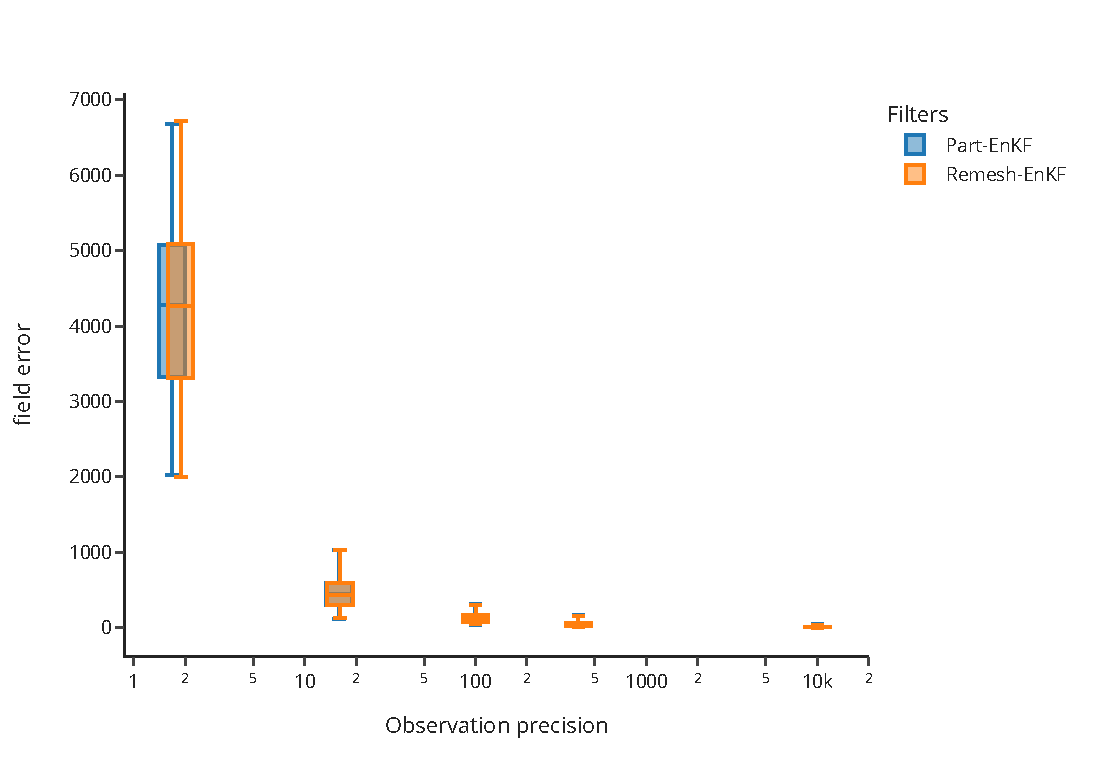
\includegraphics[width=\linewidth]{./images/app2d/final/MSE_obs_precision_box.pdf}
        \caption{}
        \label{fig:obs_precision_1}
    \end{subfigure}
    \begin{subfigure}{0.49\linewidth}
        \centering
        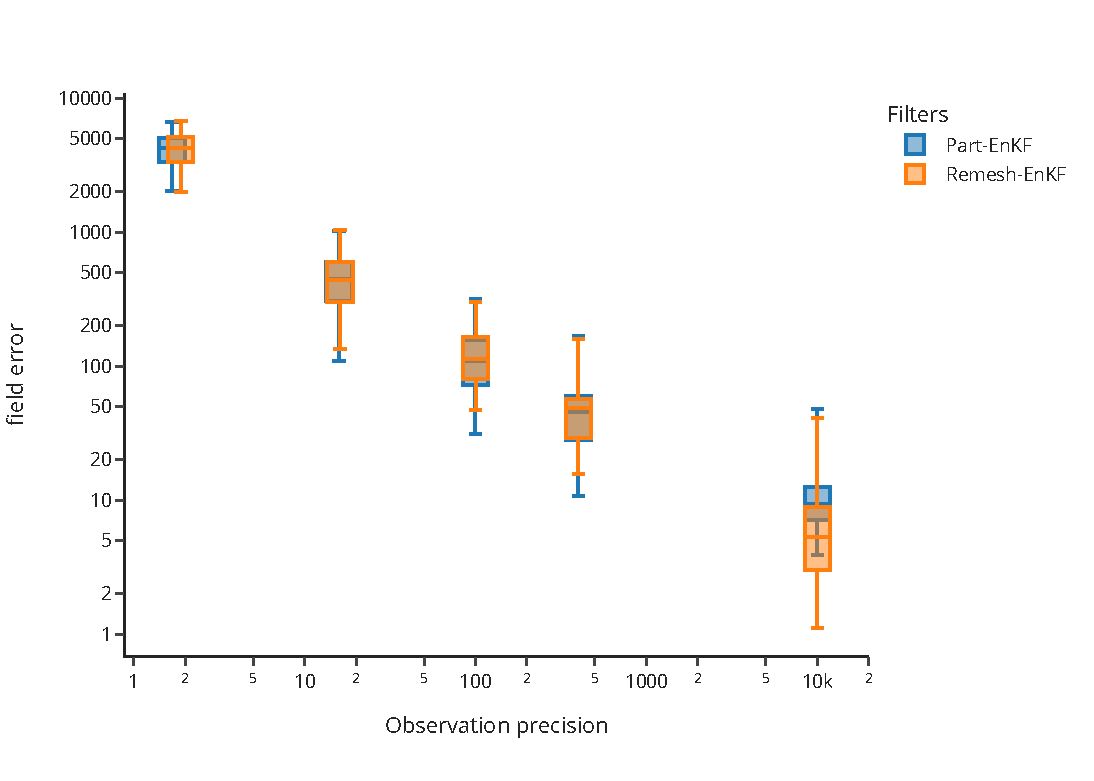
\includegraphics[width=\linewidth]{./images/app2d/final/MSE_obs_precision_box_log.pdf}
        \caption{}
        \label{fig:obs_precision_2}
    \end{subfigure}
    \caption{Diagrammes en boîte de l'erreur d'état en fonction de \(1/\sigma_{\text{obs}}^2\).}
\end{figure}


Dans la Figure~\ref{fig:na_1}, la réduction de l'erreur est encore notable et montre une diminution de la variance à mesure que le nombre d'observations augmente. Dans la Figure~\ref{fig:na_2} en échelle logarithmique, la diminution de l'erreur se produit également à un rythme constant pour les deux filtres. On observe un ordre de convergence plus élevé, environ 1.8 pour le Remesh-EnKF comparé à environ 1.4 pour le Part-EnKF.

\begin{figure}[h!]
    \centering
    \begin{subfigure}{0.49\linewidth}
        \centering
        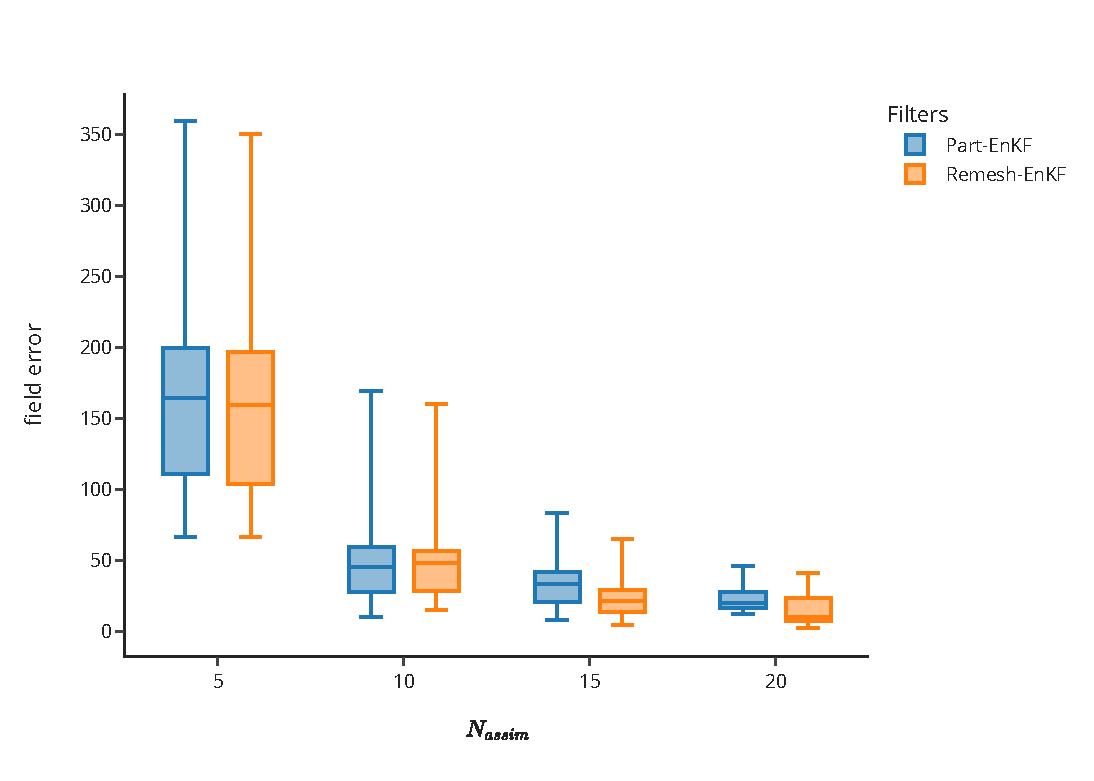
\includegraphics[width=\linewidth]{./images/app2d/final/MSE_na_box.pdf}
        \caption{}
        \label{fig:na_1}
    \end{subfigure}
    \begin{subfigure}{0.49\linewidth}
        \centering
        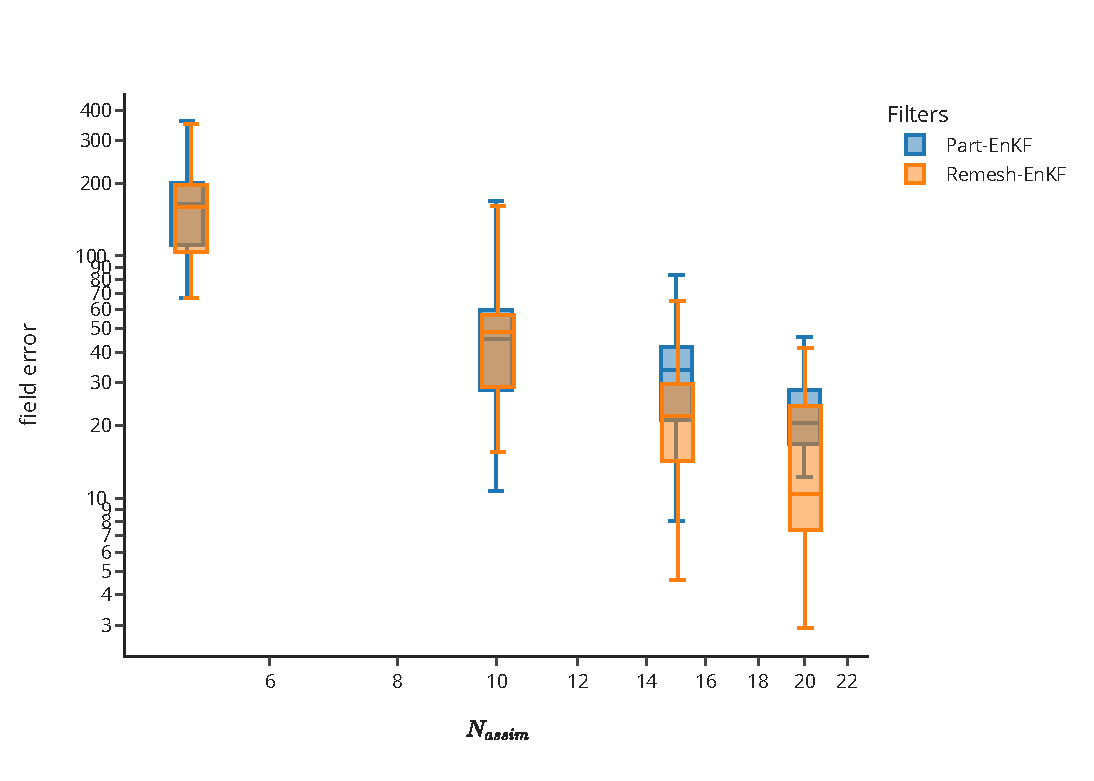
\includegraphics[width=\linewidth]{./images/app2d/final/MSE_na_box_log_log.pdf}
        \caption{}
        \label{fig:na_2}
    \end{subfigure}
    \caption{Diagrammes en boîte de l'erreur d'état en fonction de $N_{\text{assim}}$.}
    \label{fig:na}
\end{figure}

Enfin, nous analysons la convergence de l'erreur en fonction du nombre d'observations. Les emplacements des observations augmentent régulièrement sur les deux axes. Dans la Figure~\ref{fig:nobs_1}, l'estimation de l'erreur et les variances diminuent. Pour un nombre relativement faible d'observations, les deux filtres offrent des résultats similaires, tandis que le Remesh-EnKF montre des résultats relativement meilleurs lorsque le nombre d'observations est augmenté. De plus, le taux de convergence semble changer autour de 200 points d'observation, comme illustré dans la Figure~\ref{fig:nobs_2} en échelle logarithmique. Néanmoins, cela montre des performances adéquates pour les deux filtres.

\begin{figure}[h!]
    \centering
    \begin{subfigure}{0.49\linewidth}
        \centering
        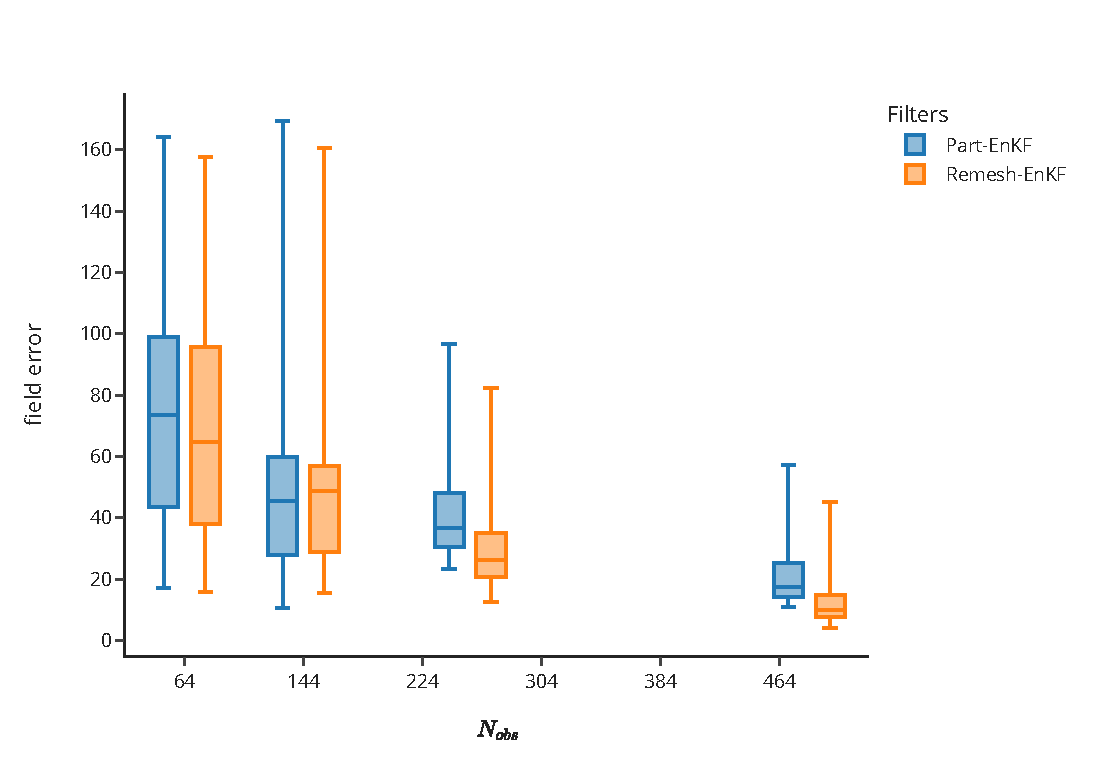
\includegraphics[width=\linewidth]{./images/app2d/final/MSE_nobs_box.pdf}
        \caption{Diagrammes en boîte de l'erreur d'état par rapport à $N_{\text{obs}}$.}
        \label{fig:nobs_1}
    \end{subfigure}
    \begin{subfigure}{0.49\linewidth}
        \centering
        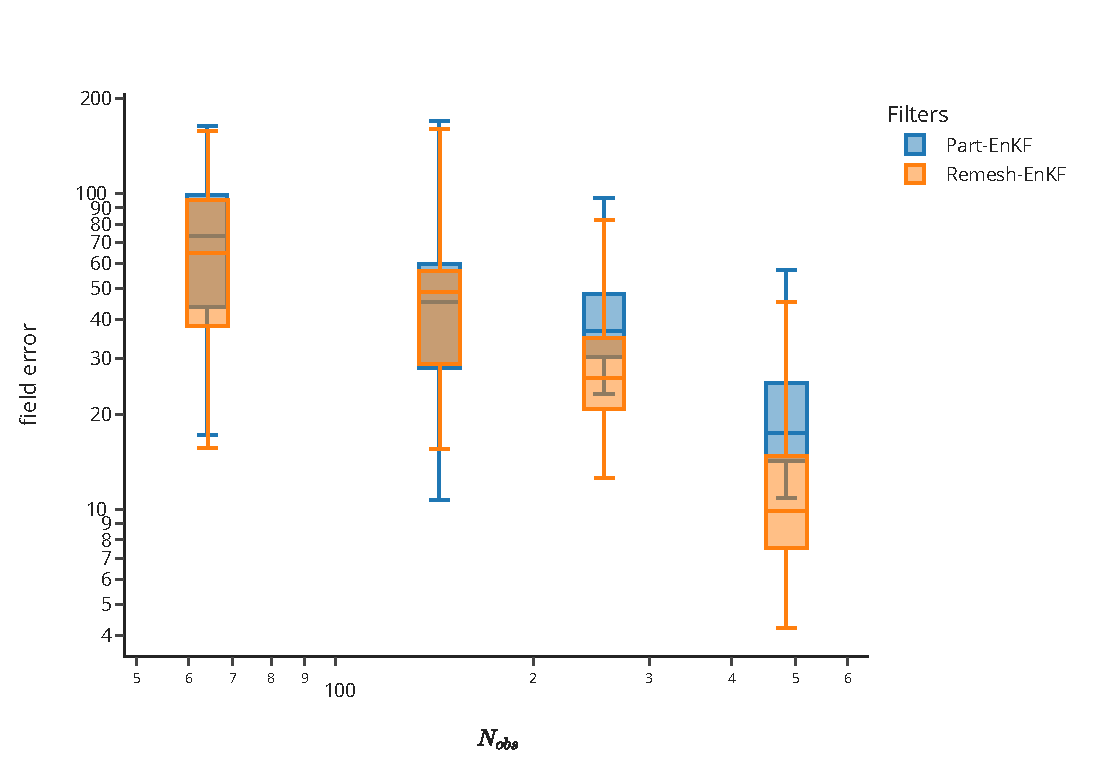
\includegraphics[width=\linewidth]{./images/app2d/final/MSE_nobs_box_log_log.pdf}
        \caption{Diagrammes en boîte de l'erreur d'état par rapport à $N_{\text{obs}}$.}
        \label{fig:nobs_2}
    \end{subfigure}
    \caption{Convergence de l'erreur par rapport au nombre d'observations. À gauche : Échelle linéaire, À droite : Échelle logarithmique.}
    \label{fig:nobs}
\end{figure}

\subsubsection{Erreur en fonction des paramètres de simulation}

Examinons maintenant l'évolution de l'erreur par rapport aux paramètres de discrétisation particulaire. Pour le Part-EnKF, il faut se rappeler que chaque membre a sa propre discrétisation de particules qui évolue selon la direction et la vitesse du dipôle et que ainsi, les résultats de se filtre sont sensibles aux paramètres de discrétisation.

Premièrement, en raison de l'irrégularité des particules dans la distribution, une approximation sévère a été introduite, ce qui a entraîné des erreurs entre la solution analysée et la solution approchée. Plus sérieusement, certaines parties de la solution peuvent disparaître car aucune particule dans le support ne peut les interpoler. Cet effet peut être observé sur plusieurs échantillons de l'ensemble où l'analyse est projetée sur une discrétisation de particules non conforme.

Par exemple, nous avons analysé la première étape d'assimilation d'un membre pour les différents filtres. Si le champ analysé est connu sur le domaine spatial, nous avons observé dans la Figure~\ref{fig
} que le Remesh-Filter et le Part-Grid-EnKF sont les seuls capables d'interpoler la solution entière. Le Part-EnKF n'est pas entièrement capable d'interpoler la solution avec la discrétisation de particules du membre prévu.

De plus, certaines distorsions observées dans la distribution des particules ne sont pas conformes au flux du champ analysé. Ces remarques sont plus critiques lorsque l'étape de prévision est plus longue, conduisant à des erreurs élevées, ou lorsque la taille du support est plus petite. De plus, l'approximation de la Section~\ref{regressionOperator} introduira l'erreur d'approximation en fonction de la taille des particules. Par exemple, la particule ne conservera pas la circulation totale en raison d'une erreur de quadrature, ce qui est le cas inverse pour le filtre Remesh-EnKF.


\section{Bilan}